\documentclass{beamer}
\setbeamertemplate{caption}[numbered]
\usepackage{animate, lipsum, subfig}

\newcommand{\comment}[1]{}

\newcommand\blfootnote[1]{%
  \begingroup
  \renewcommand\thefootnote{}\footnote{#1}%
  \addtocounter{footnote}{-1}%
  \endgroup
}

% Load Packages
\usepackage[utf8]{inputenc}
\usepackage{xcolor}
\usepackage{tikz}
\usetikzlibrary{positioning,calc}
\usepackage{graphicx}
\usepackage{hyperref}
\usepackage{amsmath}
\usepackage{listings}
%\usepackage{fontawesome}

% Define Commands
\newcommand*{\ClipSep}{0.06cm} %To adjust footer logo
\newcommand{\E}{\mathrm{e}\,} %\def\I{e} % used to defined e for exp(x), see later what it should be
\newcommand{\ud}{\mathrm{d}}
\lstset{numbers=left, numberstyle=\tiny, stepnumber=1,firstnumber=1,breaklines=true,
    numbersep=5pt,language=Python,
    stringstyle=\ttfamily,
    basicstyle=\footnotesize, 
    showstringspaces=false
}

\usetheme{oxonian}

\title{LXe scintillation model}
\begin{document}

{\setbeamertemplate{footline}{} 
\frame{\titlepage}}

\begin{frame}{Objective}
The goal is is build a scintillation model for LXe: $Y_{a}(t,\hat{\theta})$.\\
$Y_{a}(t,\hat{\theta})$ is the probability to emit a photon at time $t$ to the direction $\hat{\theta}$. The subscript $a$ indicates the different type of interactions ($\gamma$, $N$, $\alpha$ and maybe different energies in the same interaction type).\\
\end{frame}


\begin{frame}{Signal Reconstruction}
	\begin{center}
	\animategraphics[loop,controls,width=0.6\linewidth]{10}{recon-}{0}{41}	
	\end{center}
To study the temporal structure of the photon emission a processing algorithm uses a template of the average SPE signal to reconstruct the temporal PE pattern in each event for each PMT separately. The output of this process is the number of PEs created in the PMT in each digitization point.

\begin{figure}[h]
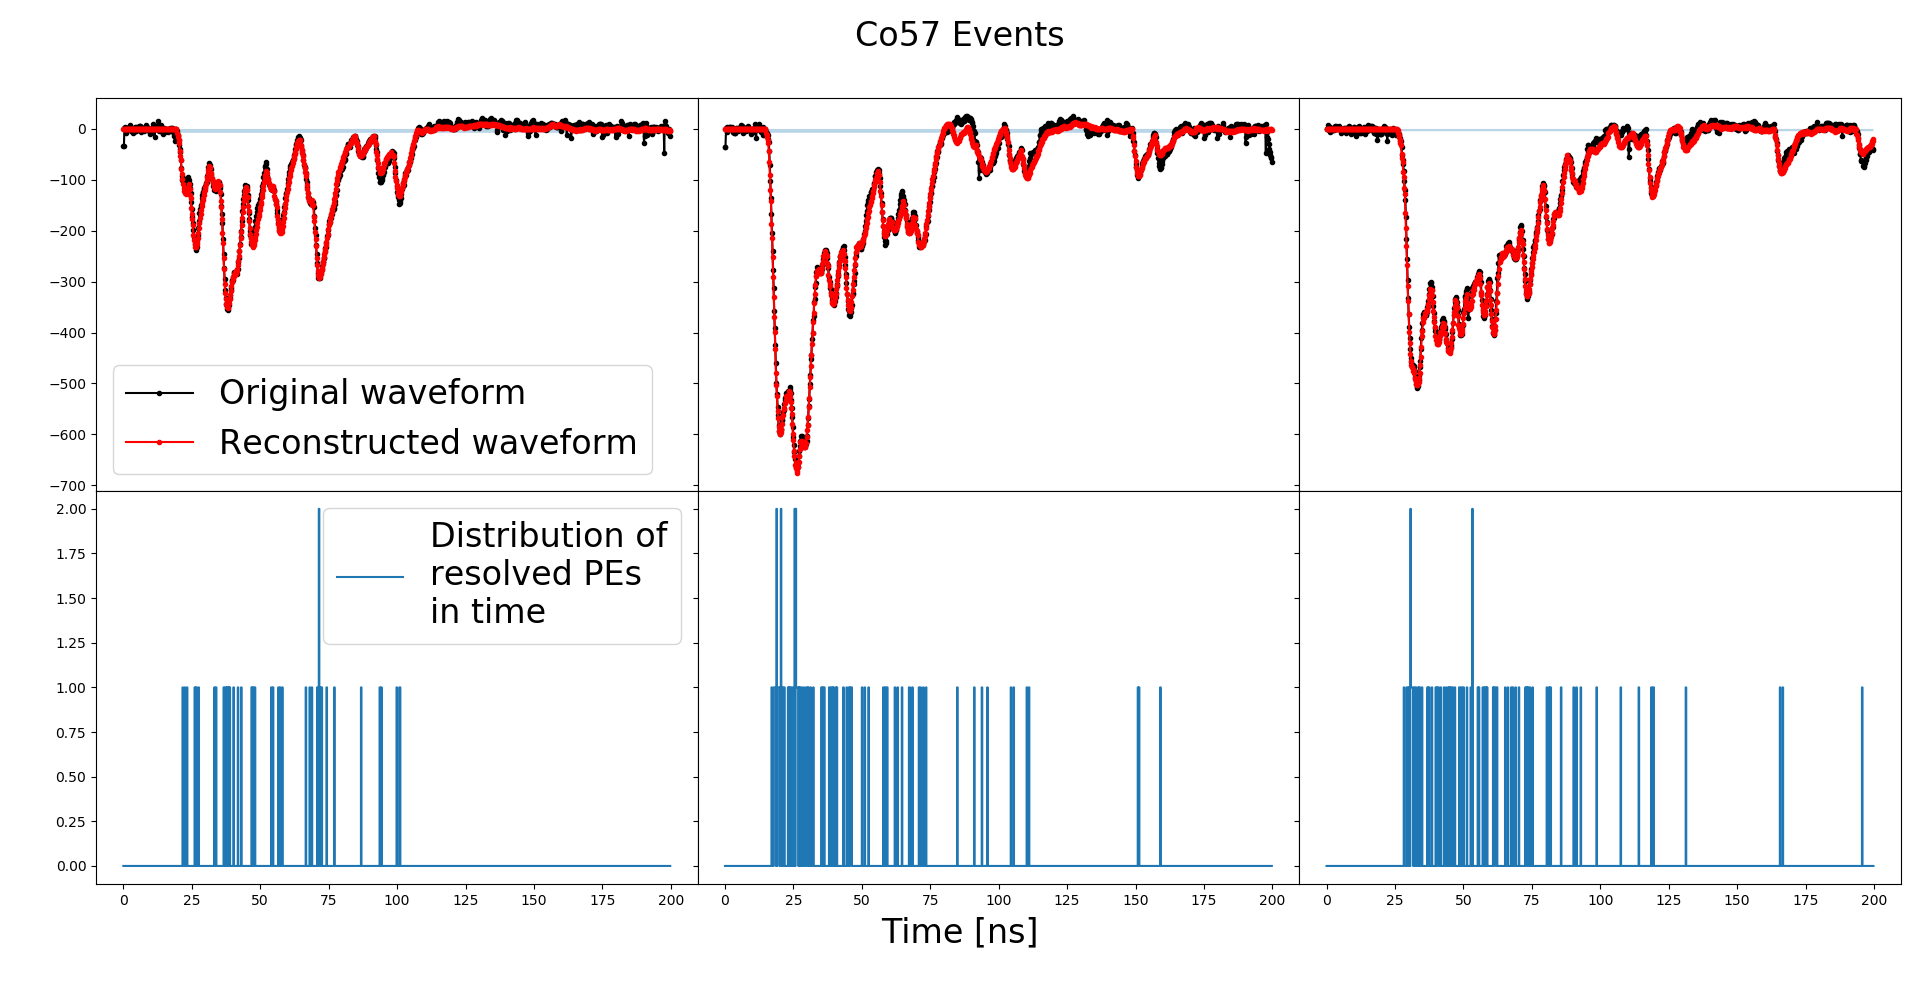
\includegraphics[width=1\textwidth]{recons.png}
\end{figure}
\end{frame}

\begin{frame}{The Dataset $D_{ni}$}
From the collection of PE times we build a dataset for each PMT - $D_{ni}$. This is a 2D table which holds the number of times $n$ PEs were resolved at time $t_i$.\\
This invokes a time alignment problem between different events.


\end{frame}

\begin{frame}{Time Alignment Problem}
We do not know the "time zero" for each event due to two reasons:\\
\begin{itemize}
\item The trigger time is "random" so alignment by the trigger time would not help.
\item Alignment by the first resolved PE in the events: the resolved PE time distribution is a random sample of the real emission times. We do not know the delay between the first resolved PE and the first photon that been emitted.
\end{itemize}
\begin{figure}[h]
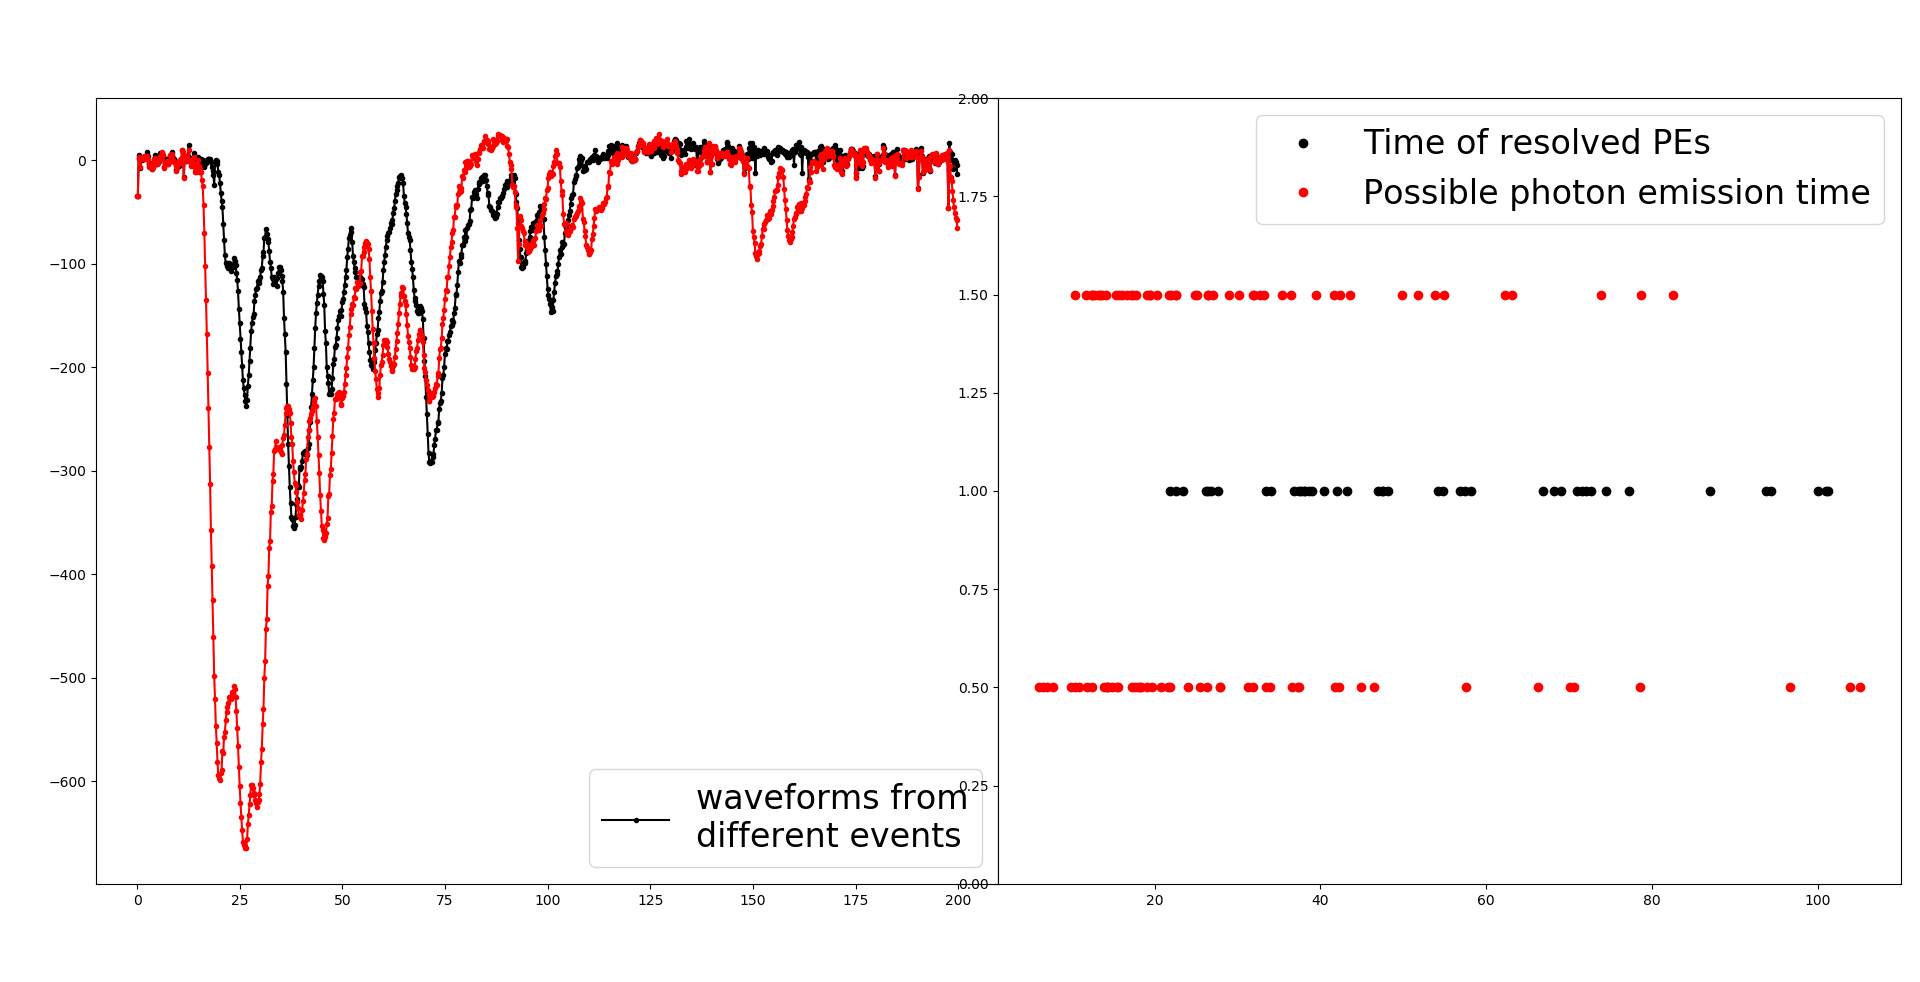
\includegraphics[width=0.7\textwidth]{alignment.png}
\end{figure}
\end{frame}

\begin{frame}{Time Alignment Problem}
Solution: Align all PMTs by the first resolved PE in the event and adjust the model from probabilities of photon emission times to probabilities of time difference between photons.  
\begin{figure}[h]
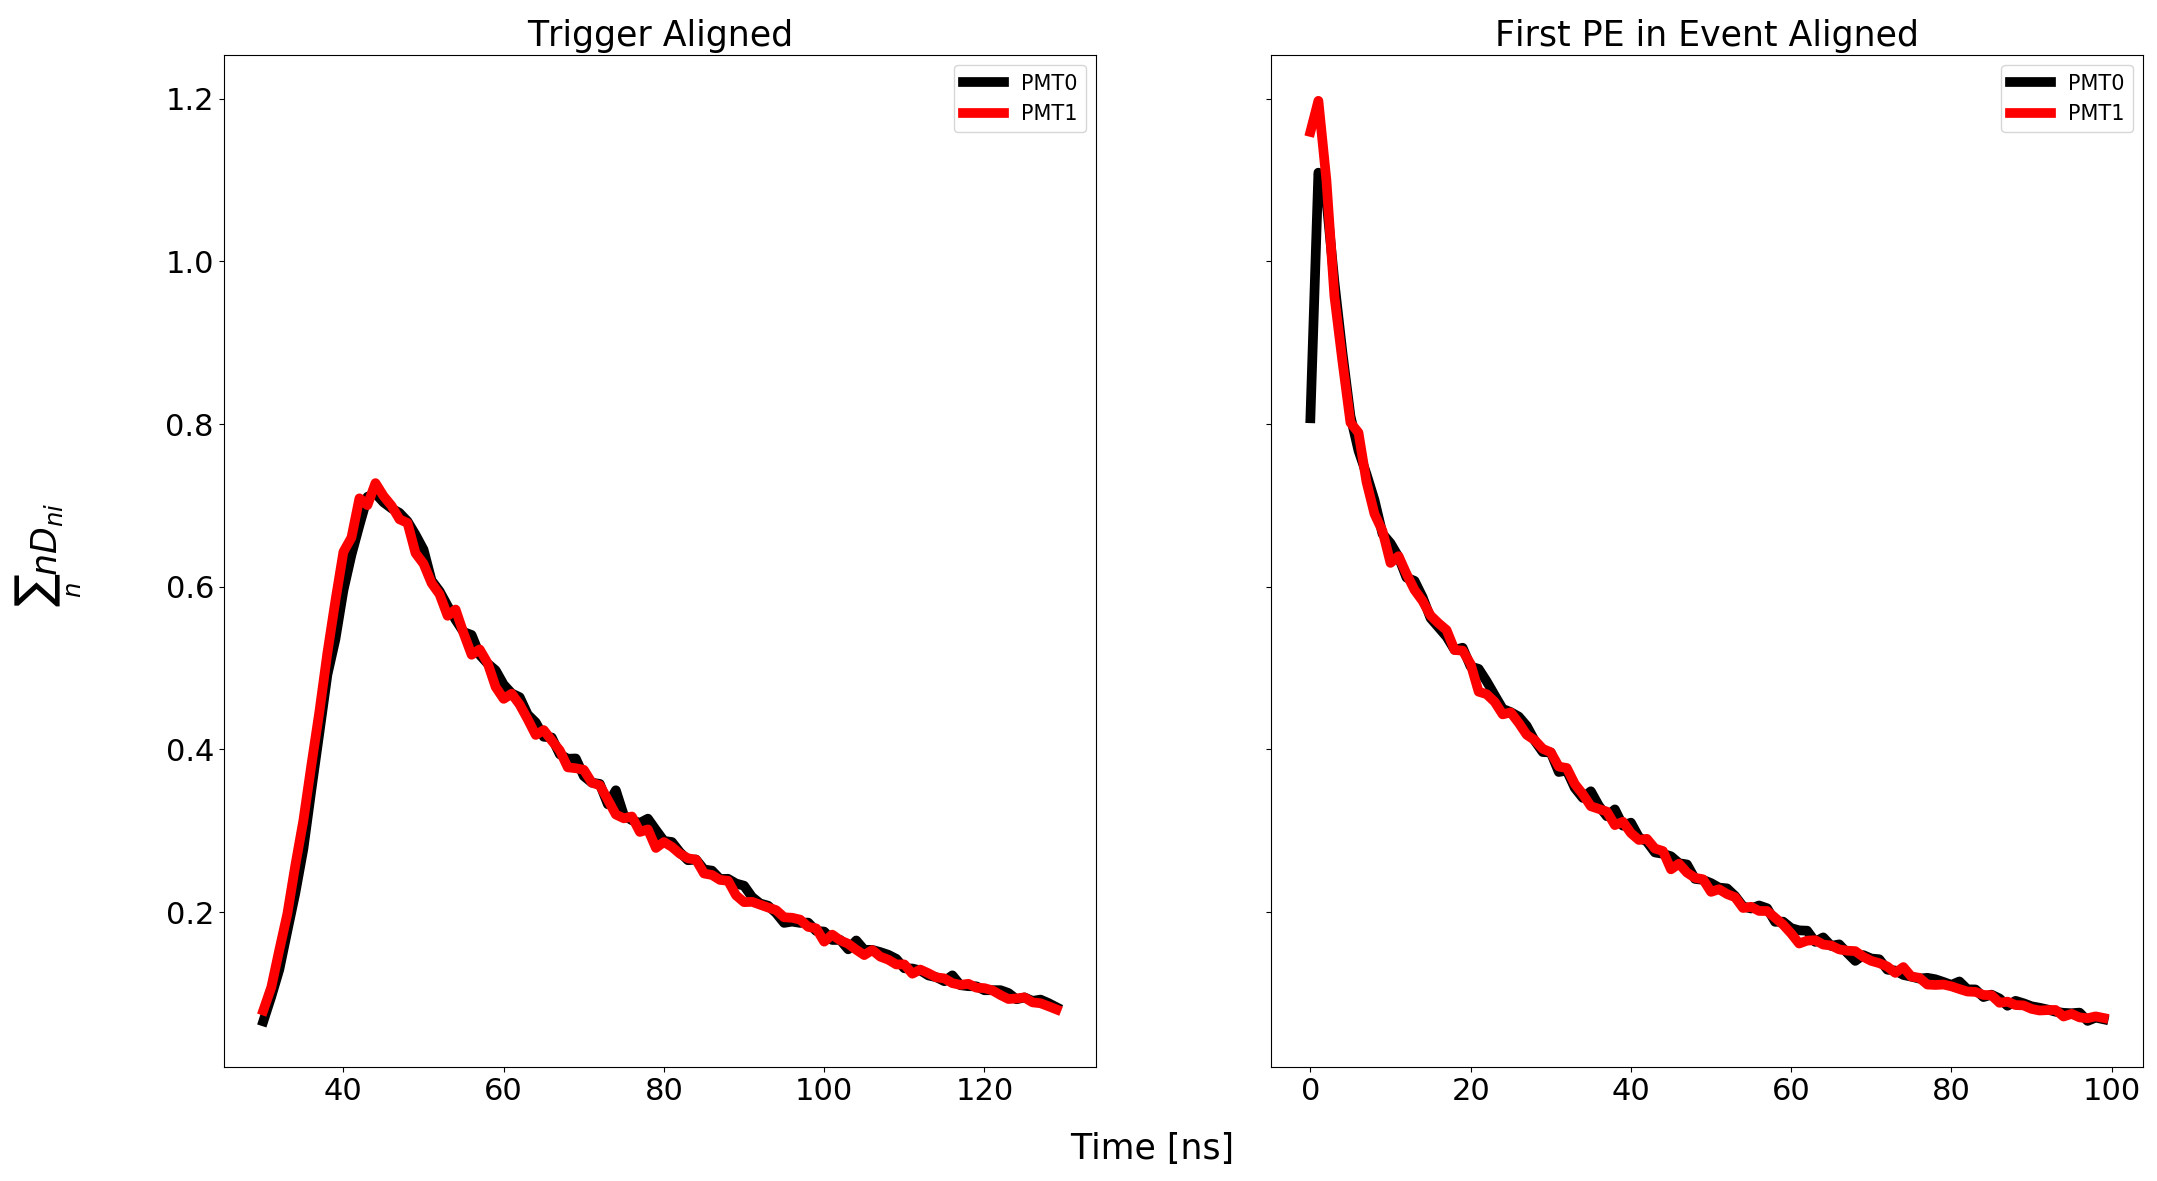
\includegraphics[width=0.73\textwidth]{sim.png}
\label{sim_temp}
\caption{Mean temporal distribution of 10K simulated events with two PMTs, double exponential decay model, 1 ns binned. Left - the fast component is smeared by the jitter of the trigger. Right - The sub-nanosecond misalignment between the two PMTs manifests itself as greater probability to resolve a PE in one PMT then in the other in the first couple of nanoseconds.}
\label{sim_temp} 
\end{figure}
\end{frame}

\begin{frame}{Data}
This is how the temporal distribution from $^{57}$Co events looks like on two PMTs (1 ns binned):
\begin{figure}[h]
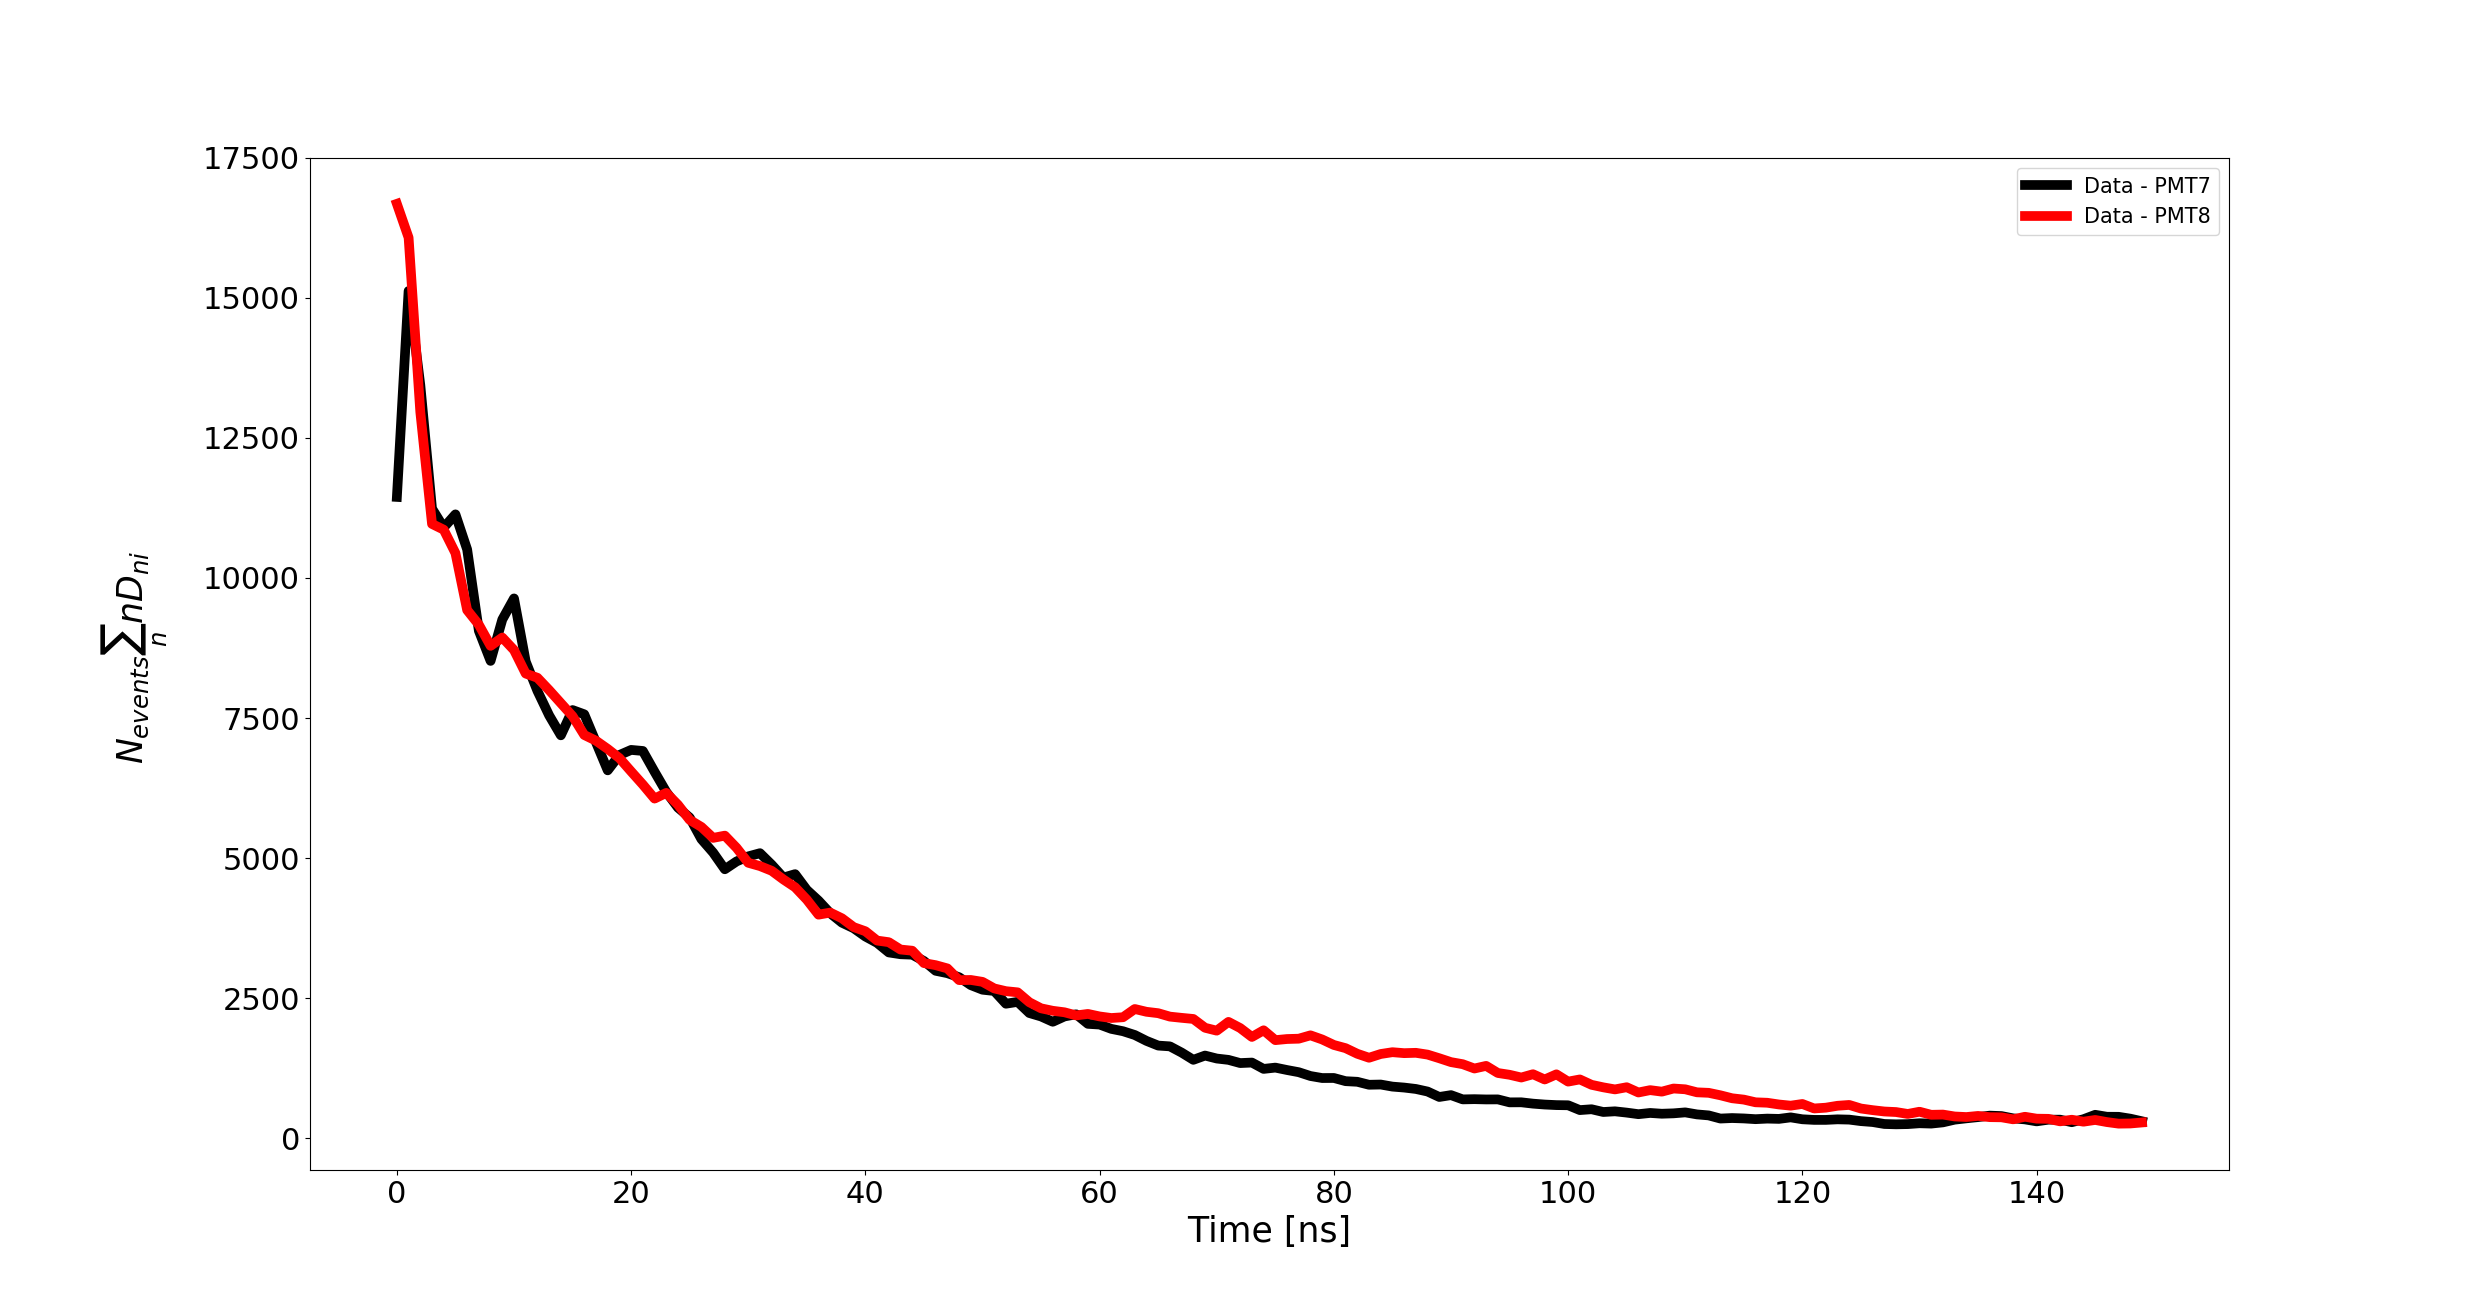
\includegraphics[width=1\textwidth]{data.png}
\end{figure}
\end{frame}

\begin{frame}{What was Wrong in the Previous Analysis}
\begin{figure}[h]
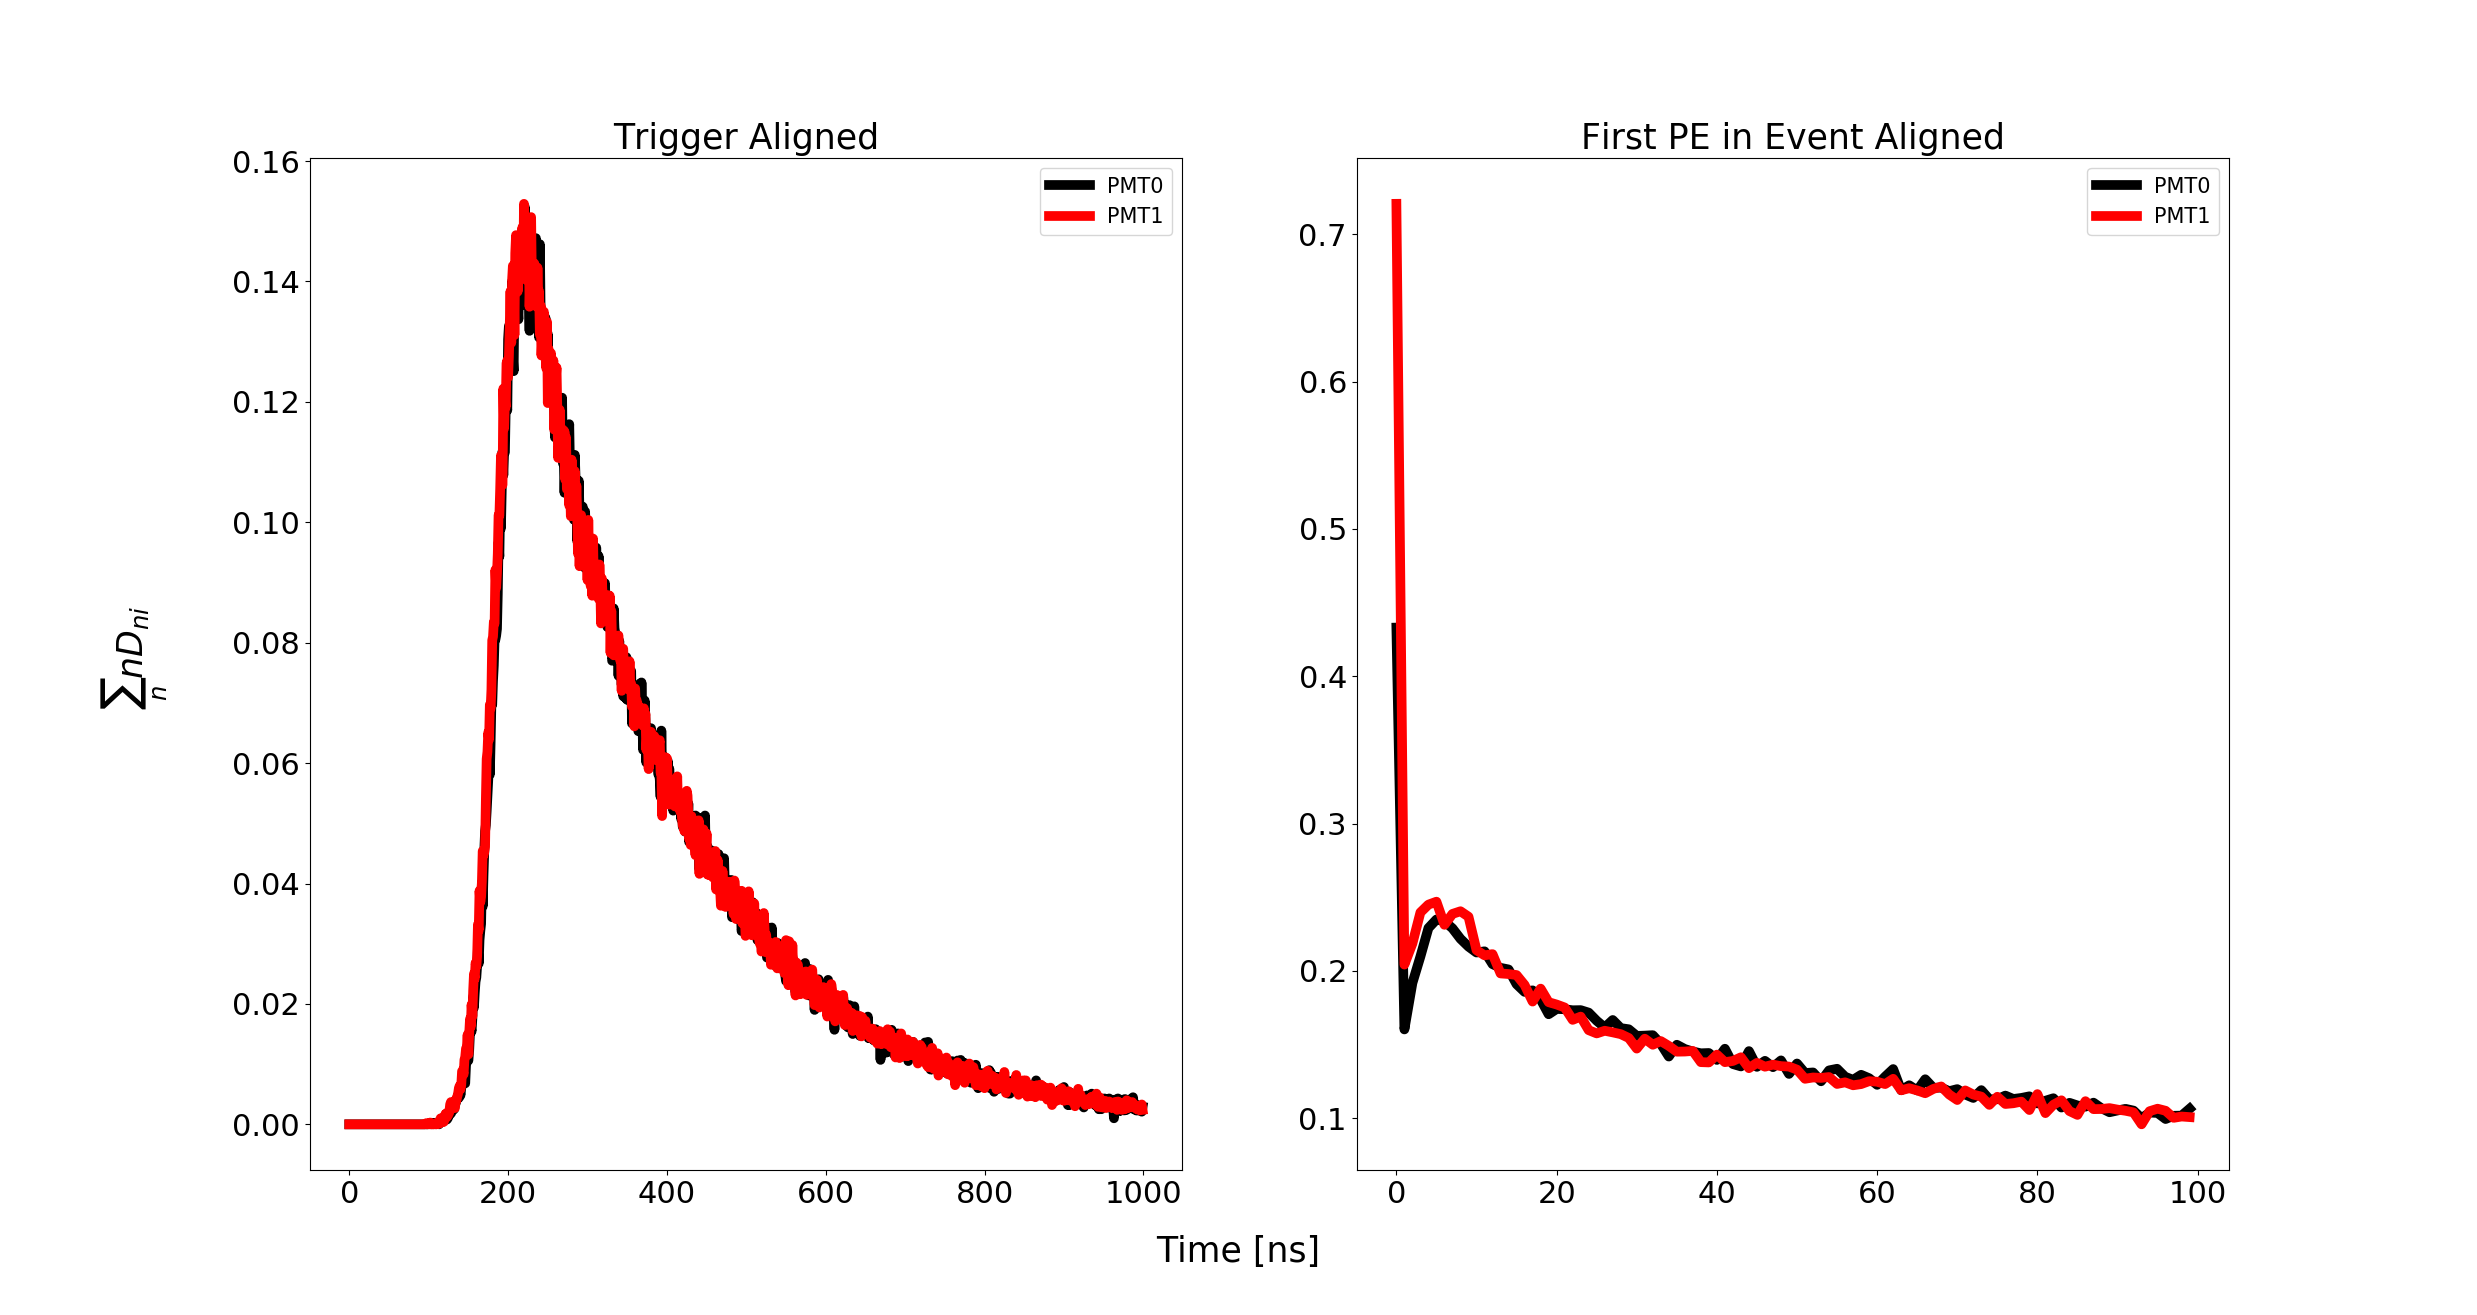
\includegraphics[width=0.8\textwidth]{sim1000.png}
\caption{This is the same simulation 0.2 ns binned. The pole in the aligned temporal structure is due the alignment by first PE - by definition we have atleast one PE at time 0. In the previous analysis I aligned the events by the time the reached 10$\%$ of their height, which is like alignment by the fist PE with some smearing. This lead to a fake $\delta$ peak. I found this systematic by simulating double exponential decay events that also gave the face $\delta$. To prevent this the development of the analyticity model should go hand-in-hand with simulation.}
\end{figure}
\end{frame}

\begin{frame}{Event Simulation}
the simulation creates the temporal structure of 10K events on two PMTs. Align the events by the first PE and finally creates a simulated 2D table for each PMT ($S_{ni}$) which holds the number of simulated events in which $n$ PEs were created at time $t_i$ after the first PE in the event. 
For each simulated event:
\begin{itemize}
\item A trigger time ($t_{trig}$) is randomly chosen from a normal distribution with mean 0 and variance $\sigma_{trig}^2$. This trigger is common for all PMTs.
\item For each PMT a total number of PEs in event ($n$) is randomly chosen out of a Poisson distribution with mean $NQ$.
\item For each PMT the $n$ PEs are grouped in two groups $n_f, n_s$ (three groups with $n_\delta$ if we want to simulate a $\delta(t)$ pulse). The occupancy of each group chosen randomly from distribution with probabilities $F, 1-F$ (and $R_\delta^a$ for the $\delta$ model). 
\end{itemize}
\end{frame}

\begin{frame}{Event Simulation}
\begin{itemize}
\item For each PMT, $nf$ times ($t_f$) are randomly chosen from an exponential distribution with decay constant $\tau_f$, and $ns$ times ($t_s$) are randomly chosen from an exponential distribution with decay constant $\tau_s$.
\item For each PMT we smear the two exponential component by shifting each sampled time $t_{f/s}^i\rightarrow \text{Normal}(\text{mean}=t_{trig}+T_0^a+t_{f/s}^i, \text{Var}=(\sigma_t)^2)$, where $\sigma_t$ is the temporal uncertainty of the PMT.
\item Find the minimal time over all PMTs (global for event) and roll all times back relative to this time.
\end{itemize}
\end{frame}

\begin{frame}{Scintillation Model}
The number of photons emitted at the time window $[t_i, t_i+dt_i]$ is distributed Poisson,
\begin{equation}
n_i^{ph}\sim\text{Poisson}(Y_a(t_i)N_adt_i)
\end{equation} 
where $N_a$ is the average number of photons generated by event type $a$ and $Y_a(t_i)$ is the probability to emit a photon at time $t_i$.
The number of PEs created in the time window is
\begin{equation}
n_i^{pe}\sim\text{Binom}(Q,\text{Poisson}(Y_a(t_i)N_adt_i)),
\end{equation}
where $Q$ is the photon detection efficiency (quantum efficiency, collection efficiency, double PE probability..., all the mechanisms that takes $m$ photons and convert them to $n<m$ PEs).
\end{frame}

\begin{frame}{Scintillation Model}
Each PMT has its temporal uncertainty combined with the code's temporal uncertainty. $\tilde{n}_i$ - the number of PEs that resolved at time window $t_i$ is a sum of a random variables $m_{ij}$ that represents the number of PEs that were created at time $t_j$ but were resolved at time $t_i$:
\begin{equation}
\begin{split}
m_{ij}&\sim n^{pe}_jdt_i\text{Norm}(t_i|T_0+t_j, \sigma_t),\\
\tilde{n}_i&\sim\sum_{j\in\text{all digi points}}m_{ij},
\end{split}
\end{equation}
where $T_0$ is the time when the events started in the digitization window and $\sigma_t$ is the temporal uncertainty of each PMT.
\blfootnote{$m_{ij}$ is kind of ill-defined with the normal distribution which gives non-integer values, but its need to be though in the sense that as the temporal uncertainty is larger there is a higher probability to resolve a bigger fraction of $n_j^{pe}$ at a different time.}
\end{frame}

\begin{frame}{Scintillation Model}
Since $\tilde{n}_i$ is a sum of independent random variables its distribution can be approximated by a different distribution with mean and variance which are the sum of the means and variances of $m_{ij}$,
\begin{equation}
\begin{split}
\langle\tilde{n}_i\rangle&=\sum_j\langle m_{ij}\rangle\\
\text{Var}(\tilde{n}_i)&=\sum_j\text{Var}(m_{ij})
\end{split}
\end{equation}
Plug in the given $n_j^{pe}$ and compute the mean and the variance of $m_{ij}$ you get
\begin{equation}
\langle m_{ij}\rangle=\text{Var}(m_{ij})=QN_adt_idt_jY_a(t_j)\text{Norm}(t_i|T_0+t_j, \sigma_t).
\end{equation}
\end{frame}

\begin{frame}{Scintillation Model}
The average and the variance of $\tilde{n}$ are equal so we assume its distributed Poisson
\begin{equation}
\begin{split}
\tilde{n}_i\sim&\text{Poisson}\left(QN_adt_idt_j\sum_jY_a(t_j)\text{Norm}(t_i|T_0+t_j, \sigma_t)\right)=\\
&\text{Poisson}\left(QN_adt_i\int Y_a(t_j)\text{Norm}(t_i|T_0+t_j, \sigma_t)dt_j\right).
\end{split}
\end{equation}
\end{frame}

\begin{frame}{Scintillation Model}
If we will take $Y_a(t_i)$ as a sum exponential decaying components
\begin{equation}
Y_a(t_j)=\sum_c\frac{F_c}{\tau_c}e^{-t_j/\tau_c} \quad (\sum_cF_c=1)
\end{equation}
we will get 
\begin{equation}
\begin{split}
&\int Y_a(t_j)\text{Norm}(t_i|T_0+t_j, \sigma_t)dt=\\
&\sum_c\frac{F_cK_c}{\tau_c}e^{-t_i\tau_c}\left[1-\text{erf}\left(\frac{\sigma_t}{\sqrt{2}\tau_c}-\frac{t_i-T_0}{\sqrt{2}\sigma_t}\right)\right]
\end{split}
\end{equation}
where $K_c$ is a normalization factor
\begin{equation}
K=\left[1-\text{erf}\left(\frac{\sigma_t}{\sqrt{2}\tau}+\frac{T_0}{\sqrt{2}\sigma_t}\right)+e^{-\sigma_t^2/2\tau^2-T_0/\tau}\left(1+\text{erf}\left(\frac{T}{\sqrt{2}\sigma_t}\right)\right)\right]^{-1}
\end{equation}
\end{frame}

\begin{frame}{Scintillation Model with $\delta(t)$}
If we want to add a super fast component in the beginning of the model it is represented by
\begin{equation}
Y_a(t)=(1-R_\delta)\sum_c\frac{F_c}{\tau_c}e^{-t/\tau_c}+R_\delta\delta(t),
\end{equation}
So we need to add to equation 8 from the previous slide:
\begin{equation}
\frac{R_\delta}{\sqrt{2\pi}\sigma_t}e^{-(t-T_0)^2/(2\sigma_t^2)}
\end{equation}
\end{frame}

\begin{frame}{Scintillation Model - Alignment}
Recall that we build a model for $H_{ni}$ which holds the number of events in which $n$ PEs were resolved at time $t_i$ after the first resolved PE.
Without the alignment problem, naively, 
\begin{equation}
\tilde{H}_{ni}=N_{\text{events}}\text{Poisson}\left(n\bigg|\lambda=QN_adt\int Y_a(t_j)\text{Norm}(t_i|T_0+t_j, \sigma_t)dt\right)
\end{equation}
\blfootnote{$\tilde{H}_{ni}$ is $H_{ni}$ before the alignment. The naively comment states that we also need to account the uncertainty in the number of PEs resolved, i.e the probability to resolve $n$ PEs where $m$ where actually extracted. This is related to the width of the SPE area distribution  and will be treated later.}
\end{frame}

\begin{frame}{Alignment for $i>0$}
The model $\tilde{H}_{ni}$ tells us what is the probability that $n$ PEs will be resolved at time $t_i$. So 
\begin{equation}
\begin{split}
H_{ni}=\sum_j&[\text{Non of the PMTs resolved a PE untill time }t_j]\times\\
&[\text{Some PMT resolved a PE (or more) at time }t_j]\times\\
&\tilde{H}_{ni+j}
\end{split}
\end{equation}
\end{frame}

\begin{frame}{Alignment for $i>0$}
\begin{equation}
\begin{split}
&[\text{Non of the PMTs resolved a PE untill time }t_j]=\\
&\prod_{\text{all PMTs}}\prod_{k<j}\tilde{H}_{0k}^{\text{pmt}}
\end{split}
\end{equation}
\begin{equation}
\begin{split}
&[\text{Some PMT resolved a PE (or more) at time }t_j]=\\
&1-\prod_{\text{pmt}}\tilde{H}_{0j}^{\text{pmt}}
\end{split}
\end{equation}

\blfootnote{The superscript pmt indicates the product on all PMTs (each pmt has a different model).}
\end{frame}

\begin{frame}{Alignment for $i>0$}
\begin{equation}
H_{ni}=\sum_j\prod_{\text{all PMTs}}\prod_{k<j}\tilde{H}_{0k}^{\text{pmt}}\left(1-\prod_{\text{pmt}}\tilde{H}_{0j}^{\text{pmt}}\right)\tilde{H}_{ni+j}
\end{equation}
\end{frame}

\begin{frame}{Alignment for $i=0, n>0$}
In this case we dont need the middle term in the previous slide (which represents the probability that the first PE was resolved at time $t_j$), So for $n>0$
\begin{equation}
H_{n0}=\sum_j\prod_{\text{all PMTs}}\prod_{k<j}\tilde{H}_{0k}^{\text{pmt}}\tilde{H}_{nj}
\end{equation}
\end{frame}

\begin{frame}{Alignment for $i=0, n=0$}
Here we do need the middle term but we dont want to sum on the pmt of interest. So
\begin{equation}
H_{00}^{\text{pmt}_0}=\sum_j\prod_{\text{all PMTs}}\prod_{k<j}\tilde{H}_{0k}^{\text{pmt}}\left(1-\prod_{\text{pmt}\neq\text{pmt}_0}\tilde{H}_{0j}^{\text{pmt}}\right)\tilde{H}_{0j}^{\text{pmt}_0}
\end{equation}
\end{frame}

\begin{frame}{First Look at Data}
I ran the reconstruction algorithm on the $^{57}$Co dataset with PMTs 7 and 8. In each event the two signals were aligned by the delay that was measured by the pulser data. After reconstruction the temporal pattern of the resolved PEs was aligned ones more relative to the first PE resolved (in PMT 7 or 8). The events in which the $\chi^2$ of the reconstructed signal relative to the signal was too big were cut out. Also events with large baseline width were cut out. A range in the energy spectrum (number of resolved PEs) of each PMT was chosen and from these events a 2D table was made for each PMT ($D_{ni}$) which holds the number of events in which $n$ PEs was resolved at time $t_i$ after the first resolved PE.
\end{frame}

\begin{frame}{First Look at Data}
\begin{figure}[h]
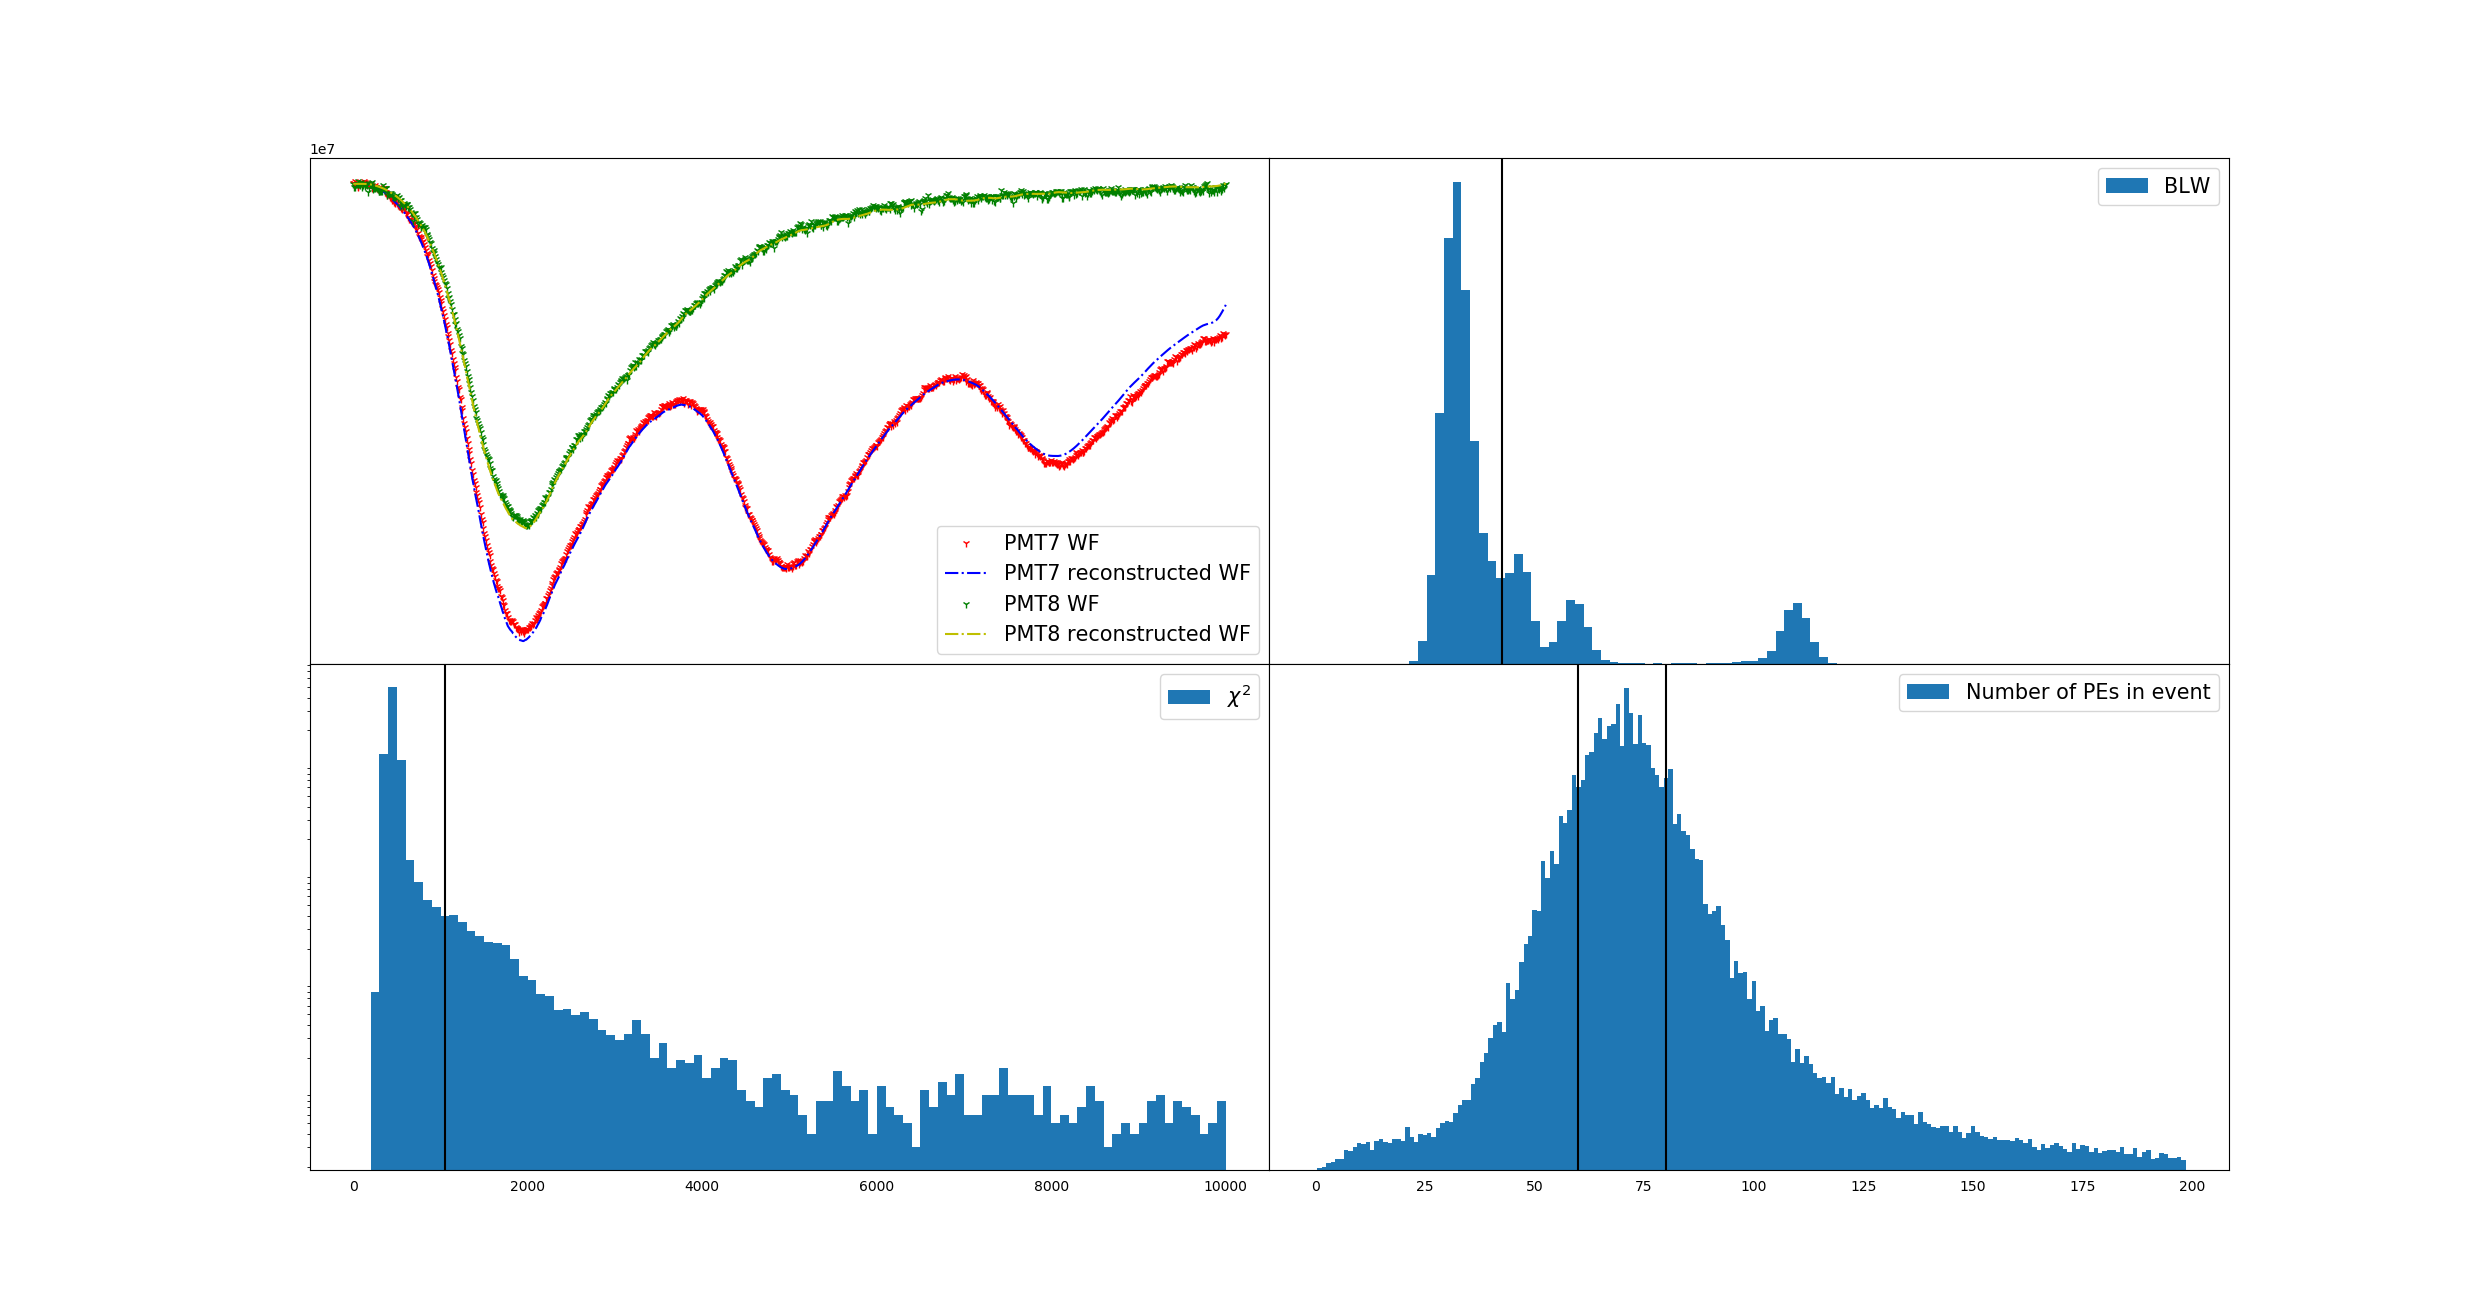
\includegraphics[width=1\textwidth]{data_event.png}
\end{figure}
\end{frame}

\begin{frame}{First Look at Fit}
\begin{figure}[h]
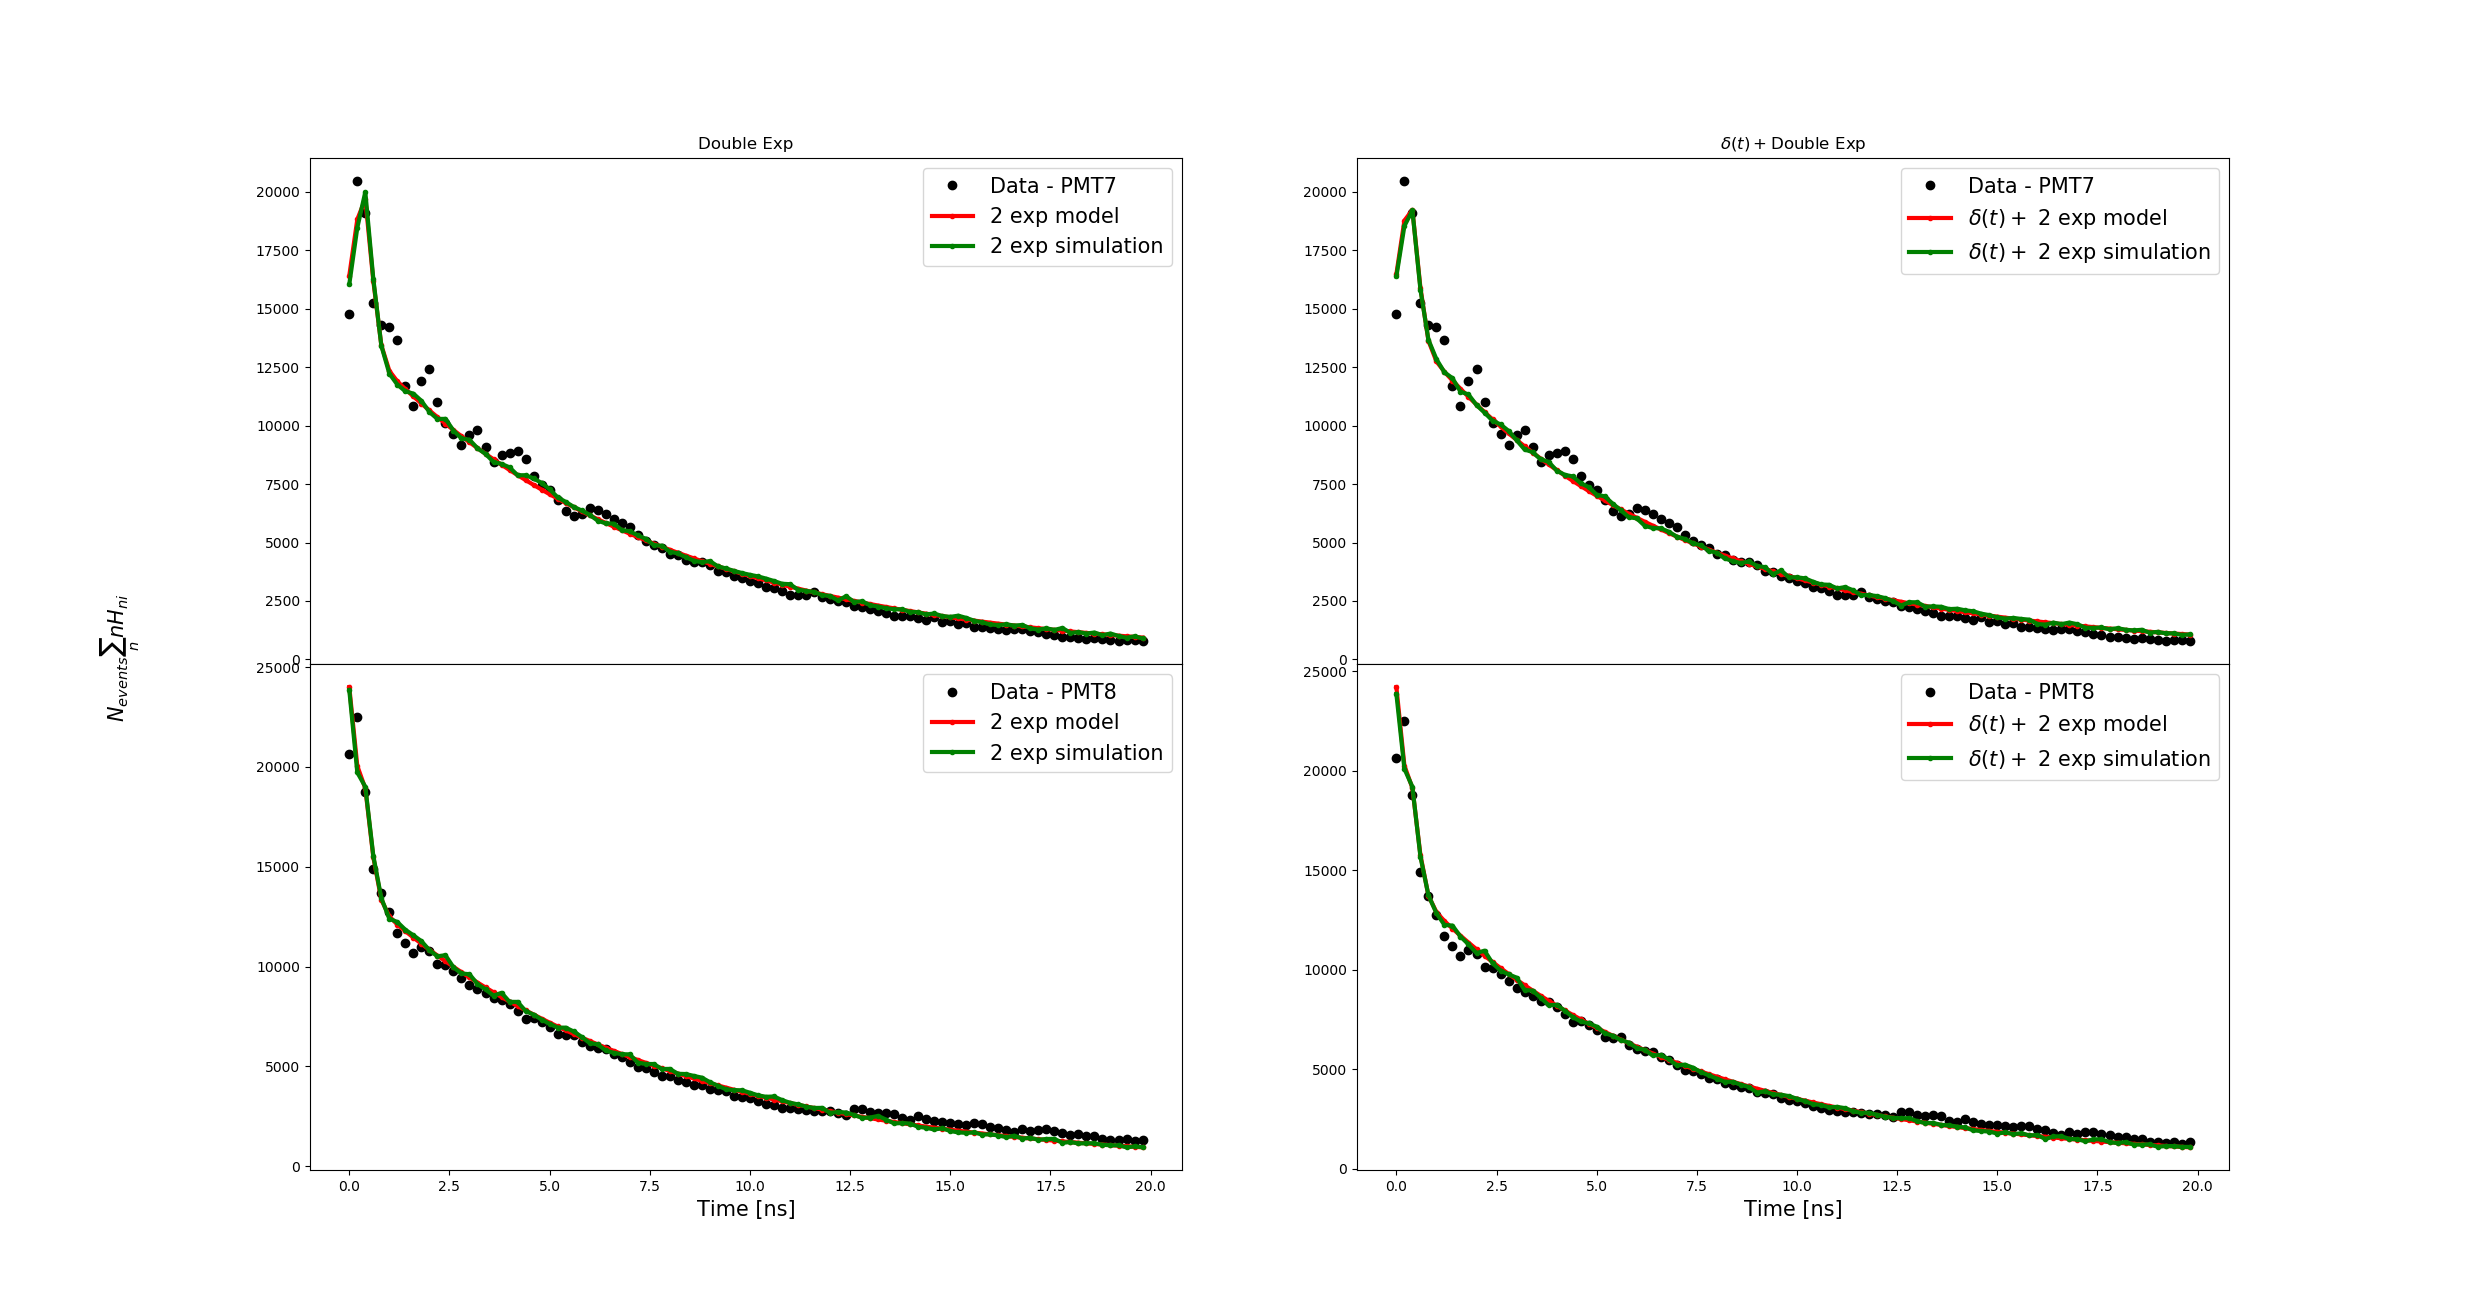
\includegraphics[width=1\textwidth]{fitA.png}
\end{figure}
First of all we see that the model and the simulation gives the same results so we can assume that the analytical model models the process we think happens.
\end{frame}

\begin{frame}{First Look at Fit}
\begin{itemize}

\item Double exp model:
\begin{center}
\begin{tabular}{|c||c|c|c|c|c|c|} 
\hline
PMT & $NQ$ & $T_0$ [ns]& $\sigma_t$ [ns] & $F$ & $\tau_f$ [ns] & $\tau_s$ [ns]\\ 
\hline\hline
7 & 34 & 39.9 & 1.01 & 0.07 & 0.19 & 36.5 \\
\hline
8 & 35 & 39.5 & 1.08 & -- & -- & -- \\
\hline
\end{tabular}
\end{center} 
It seems that the fit needs a sub-nanosecond component, but a sub-nanosecond exponential with a nanosecond smearing is identical to a $\delta$ signal.


\item $\delta(t)+$ Double exp model:
\begin{center}
\begin{tabular}{|c||c|c|c|c|c|c|c|} 
\hline
PMT & $NQ$ & $T_0$ [ns]& $\sigma_t$ [ns] & $R$ & $F$ & $\tau_f$ [ns] & $\tau_s$ [ns]\\ 
\hline\hline
7 & 36 & 45.3 & 0.9 & 0.06 & 0.7 & 30 & 100 \\
\hline
8 & 37 & 45.07 & 1.08 & 0.07 & -- & -- & -- \\
\hline
\end{tabular}
\end{center} 
Here it is seems that the $\delta$ takes most of the fast component and the $\tau_f$  represents the slow component (notice the difference of $F$ in the two models).
\end{itemize}

\end{frame}

\begin{frame}{Constraints on $\sigma_t$ and $T_0$}
We can use the delay distribution from the pulser data to help the fit.
\begin{figure}[h]
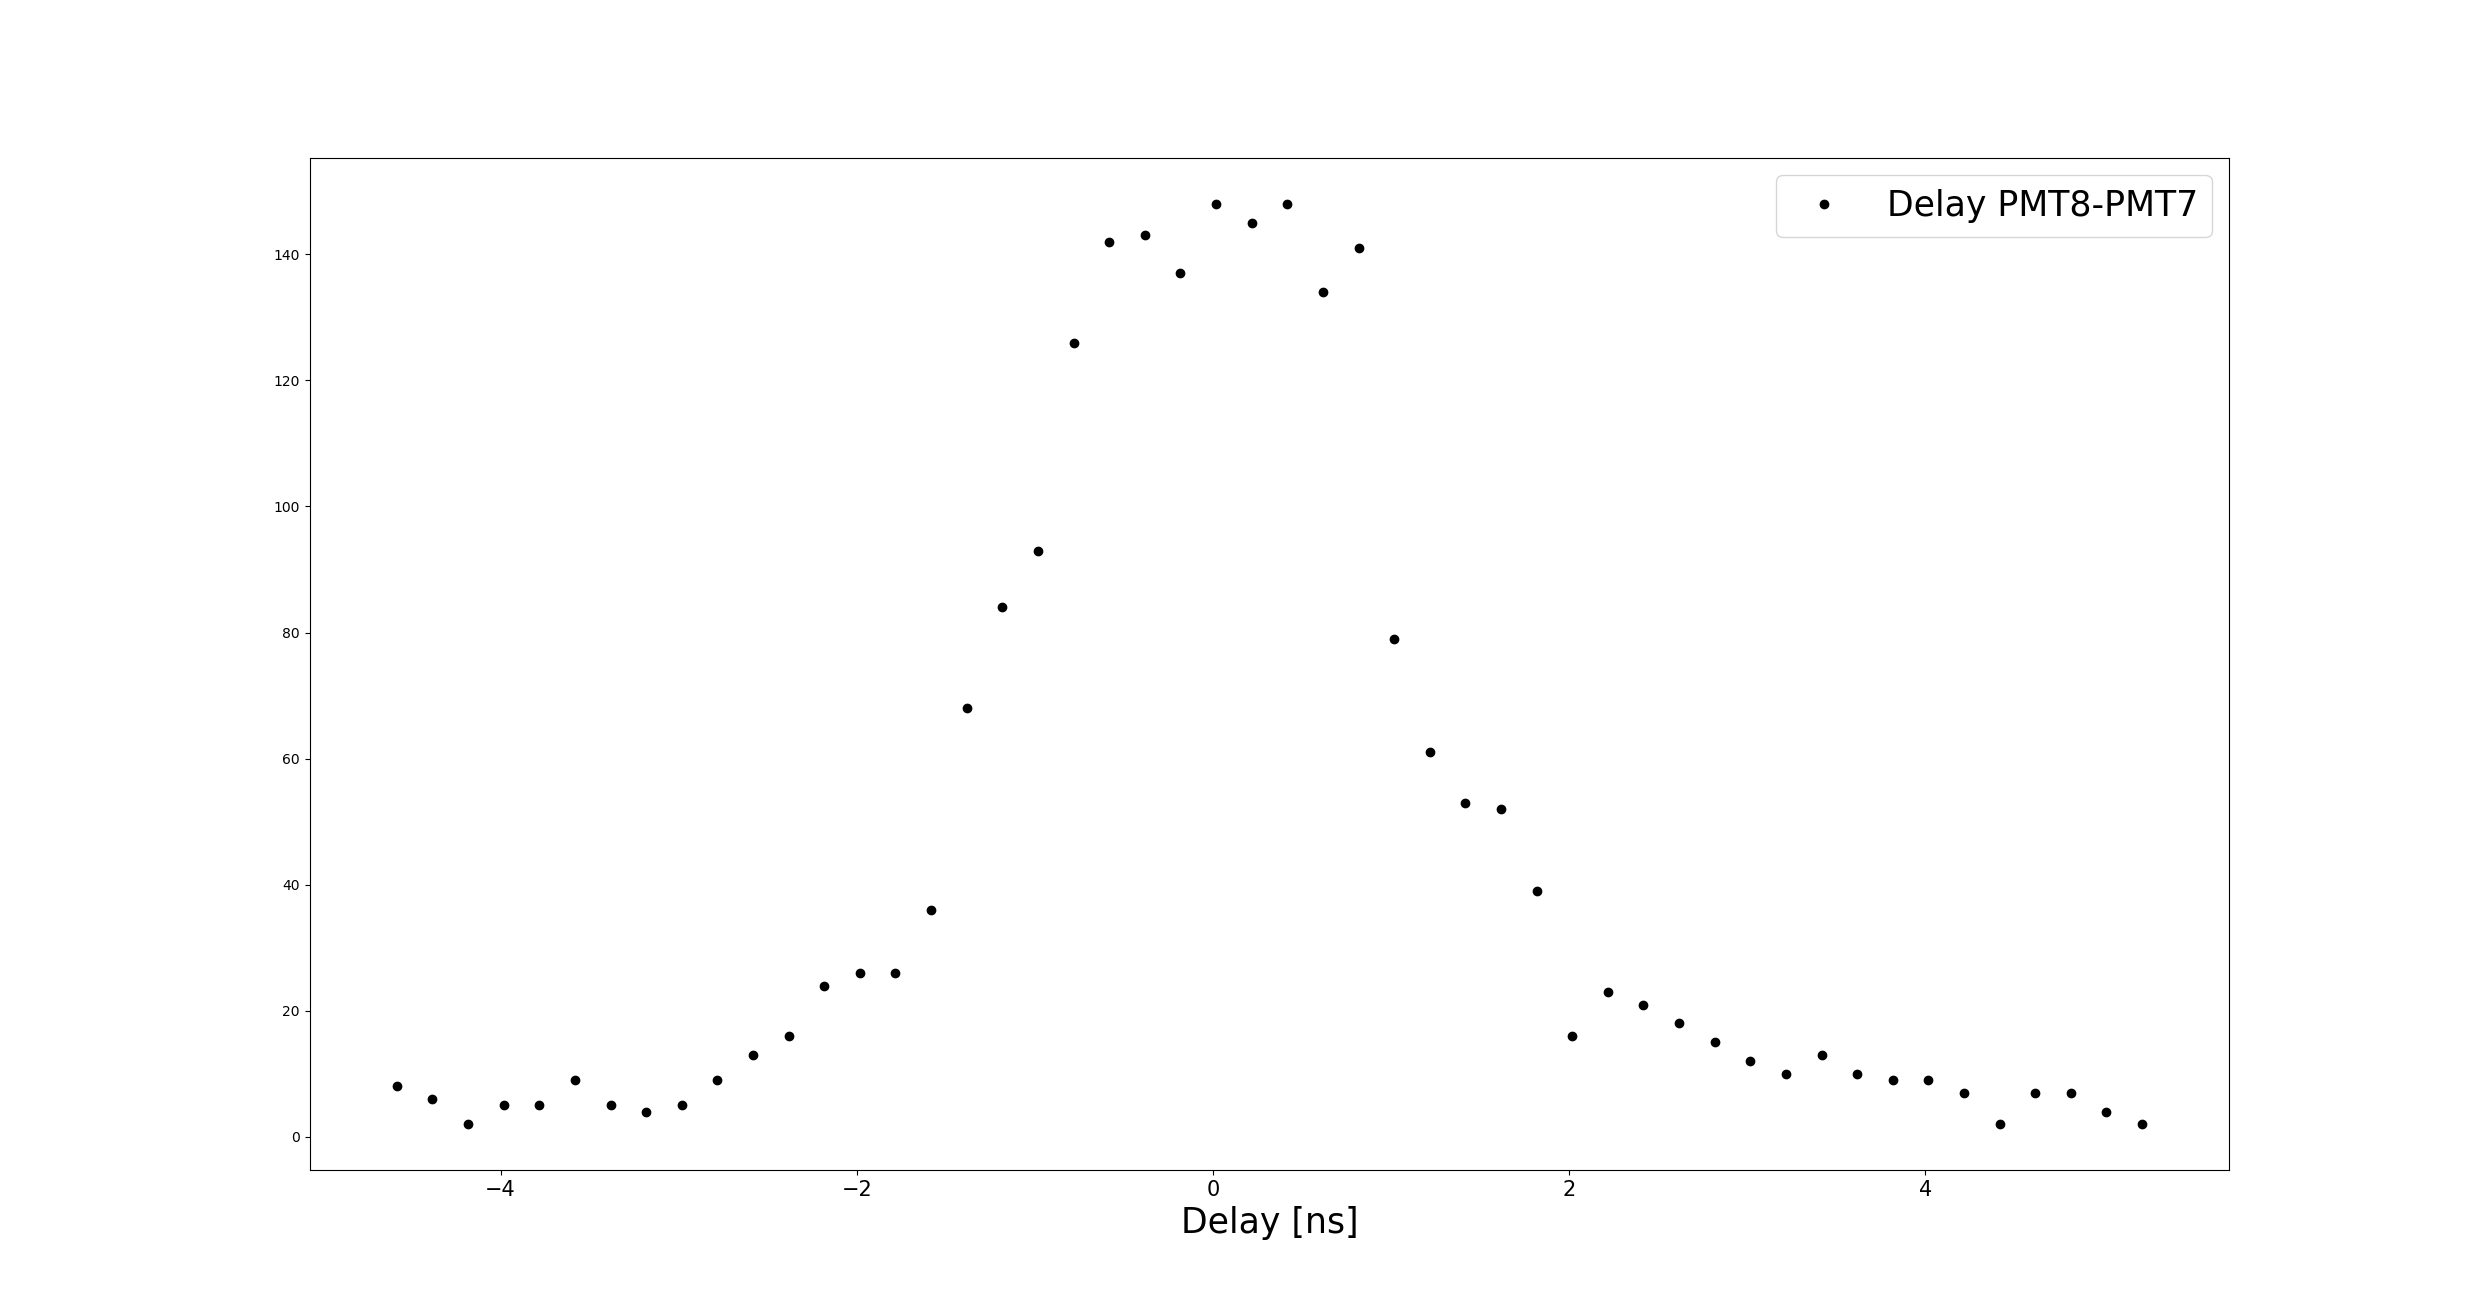
\includegraphics[width=1\textwidth]{model_delay.png}
\end{figure}
\begin{equation}
\text{Delay Distribution}^{ij}=a_{\text{delay}}^{ij}e^{-\frac{\left(\text{Delay}-(T_0^i-T_0^j)\right)^2}{2\left((\sigma_t^i)^2+(\sigma_t^j)^2\right)}}
\end{equation}
\end{frame}

\begin{frame}{Constraints on $NQ$}
We can use the number of PEs resolved in each event ("energy spectrum") to help the fit.
\begin{figure}[h]
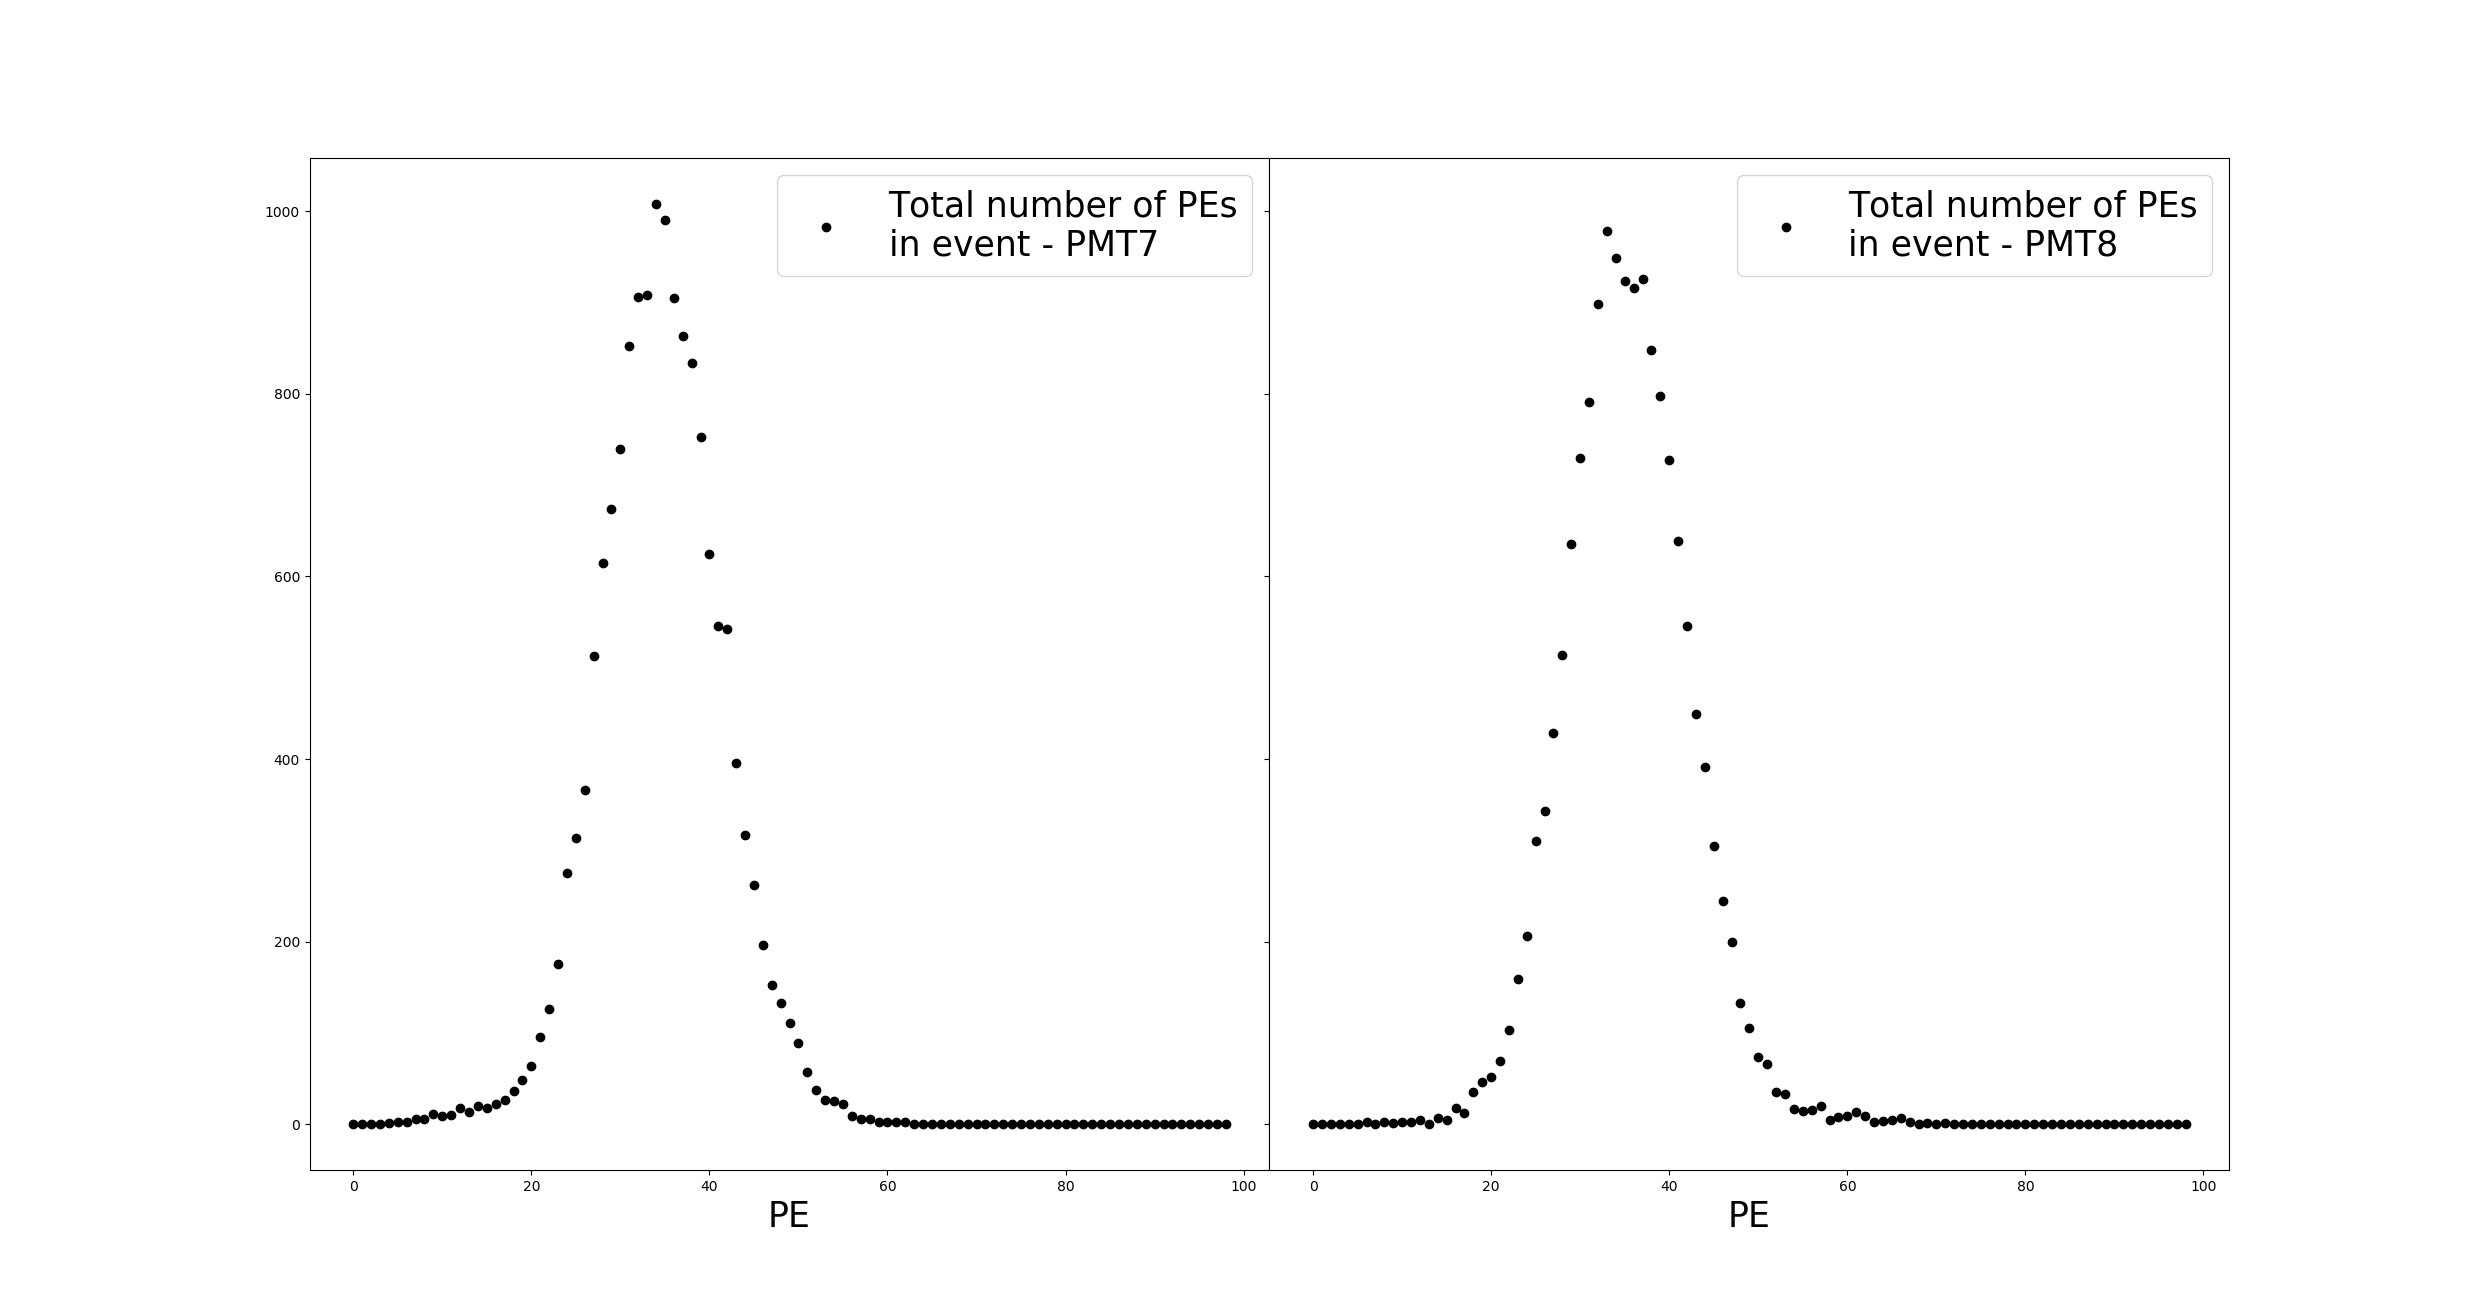
\includegraphics[width=0.8\textwidth]{totalPE.png}
\end{figure}
\begin{equation}
\begin{split}
\text{Total number of PEs in event resolved in a PMT}=\\
N_{\text{events}}\text{Poisson}\left(PE|\lambda=\sum_{ni}nH_{ni}\right)
\end{split}
\end{equation}
\end{frame}

\begin{frame}{Global Fit for the Temporal Structure the Spectra and the Delay Distribution}
\begin{figure}[h]
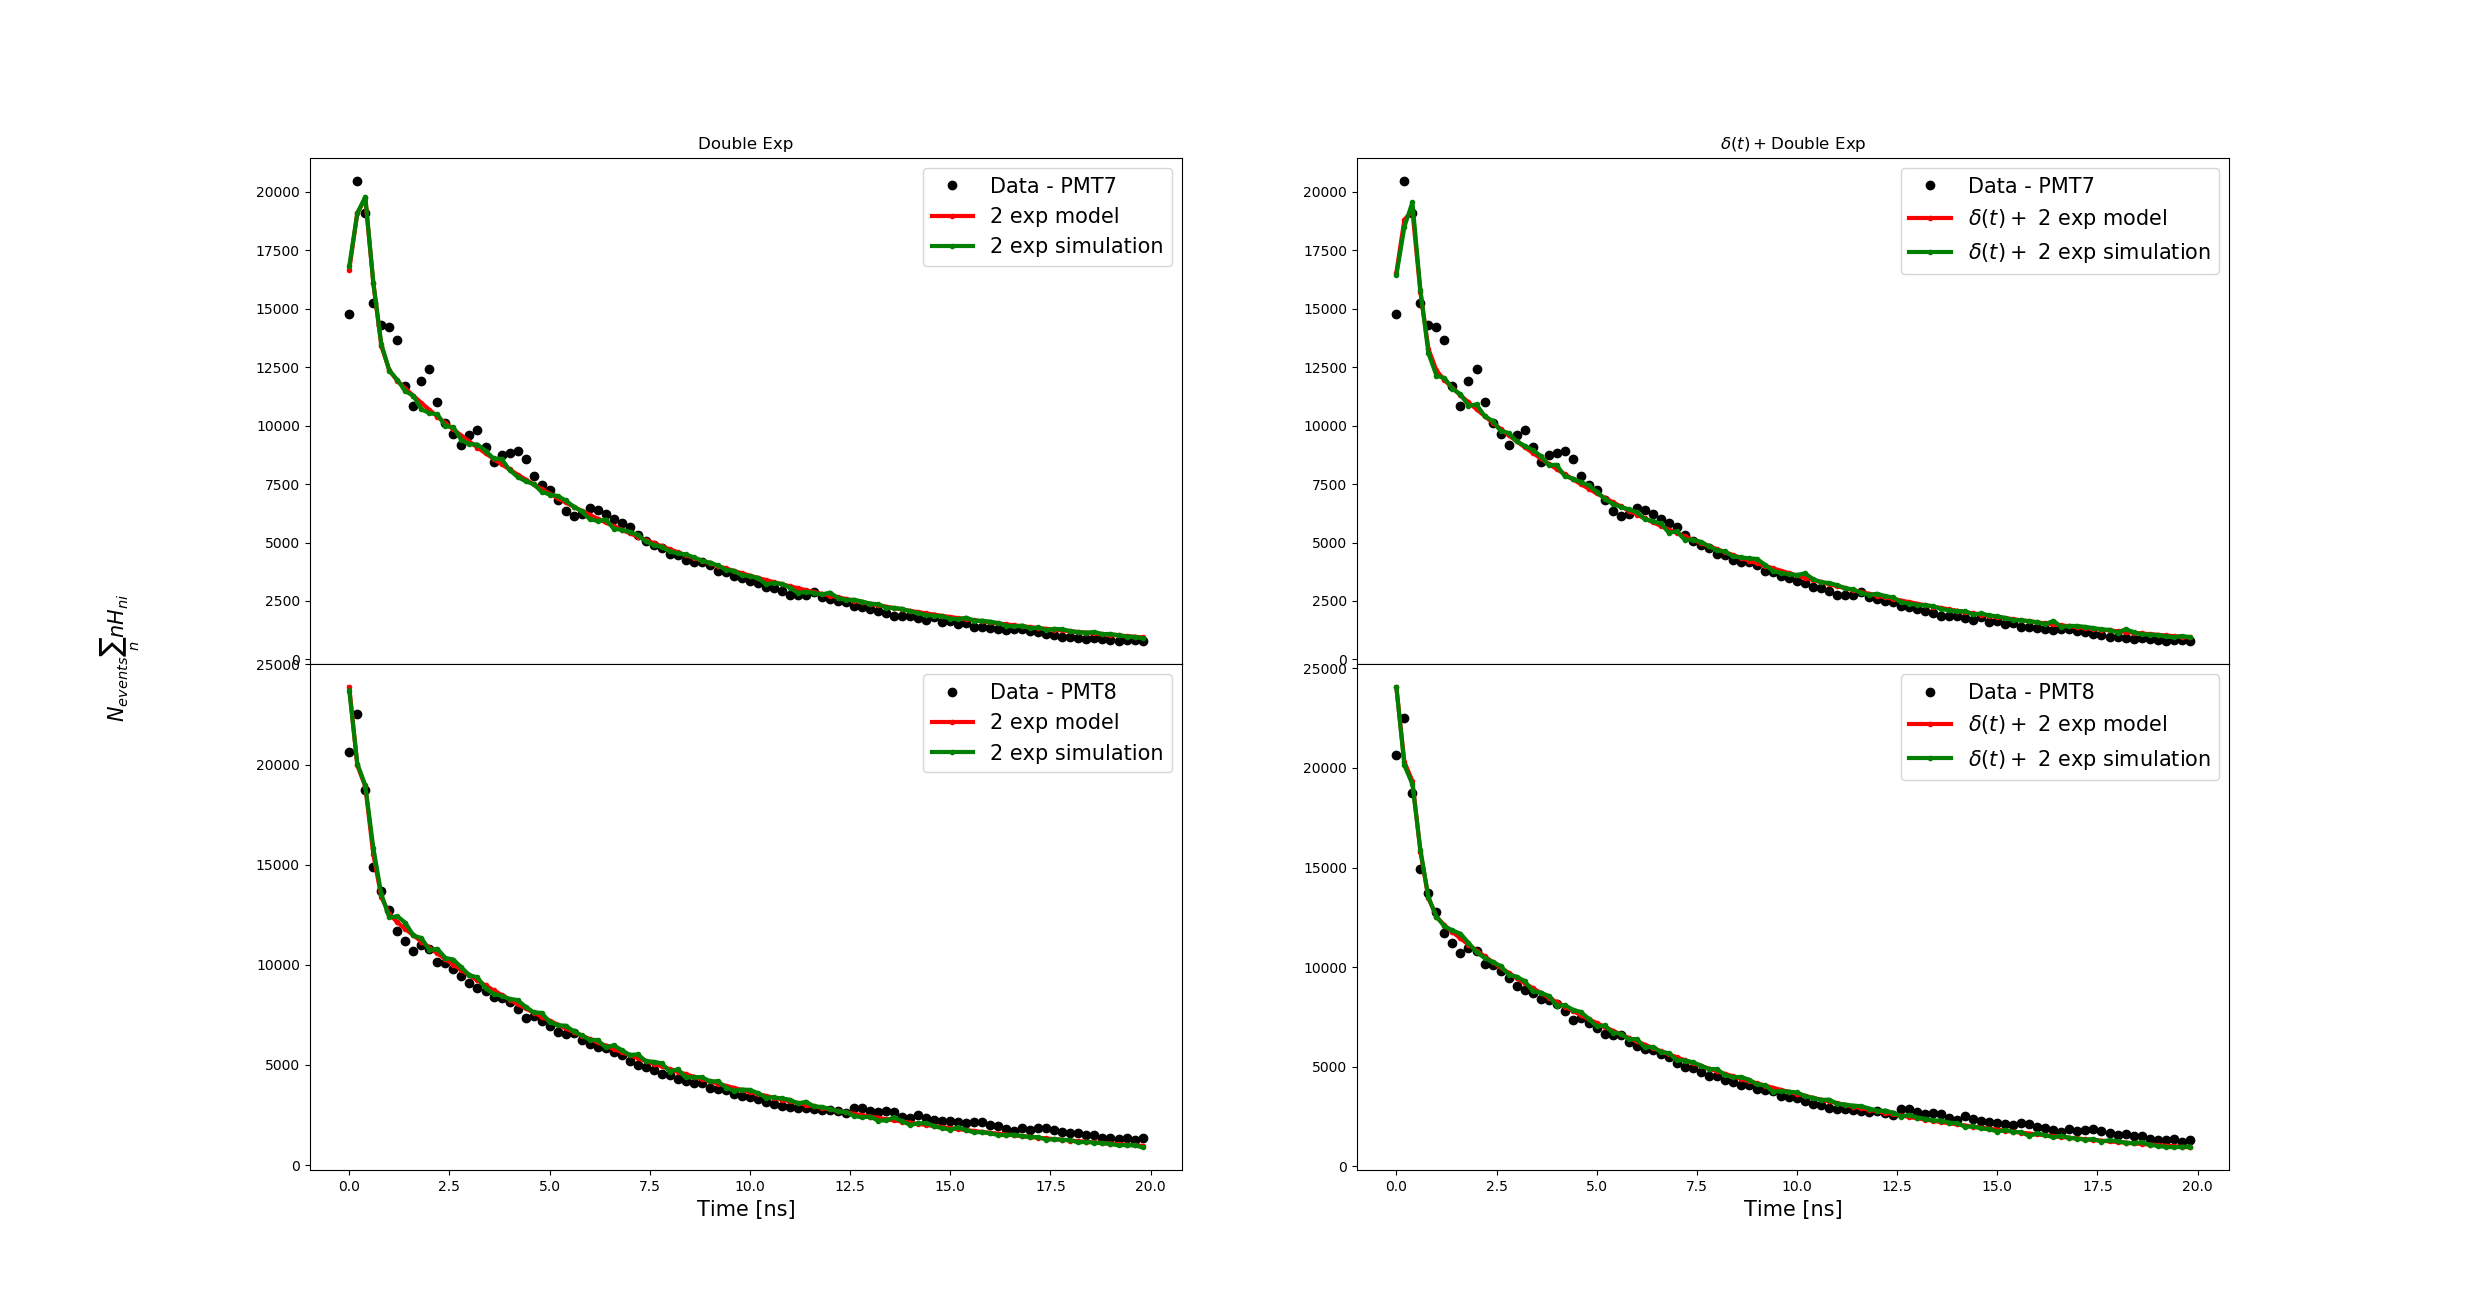
\includegraphics[width=1\textwidth]{fitB.png}
\end{figure}
\end{frame}

\begin{frame}{Global Fit for the Temporal Structure the Spectra and the Delay Distribution}
\begin{figure}[h]
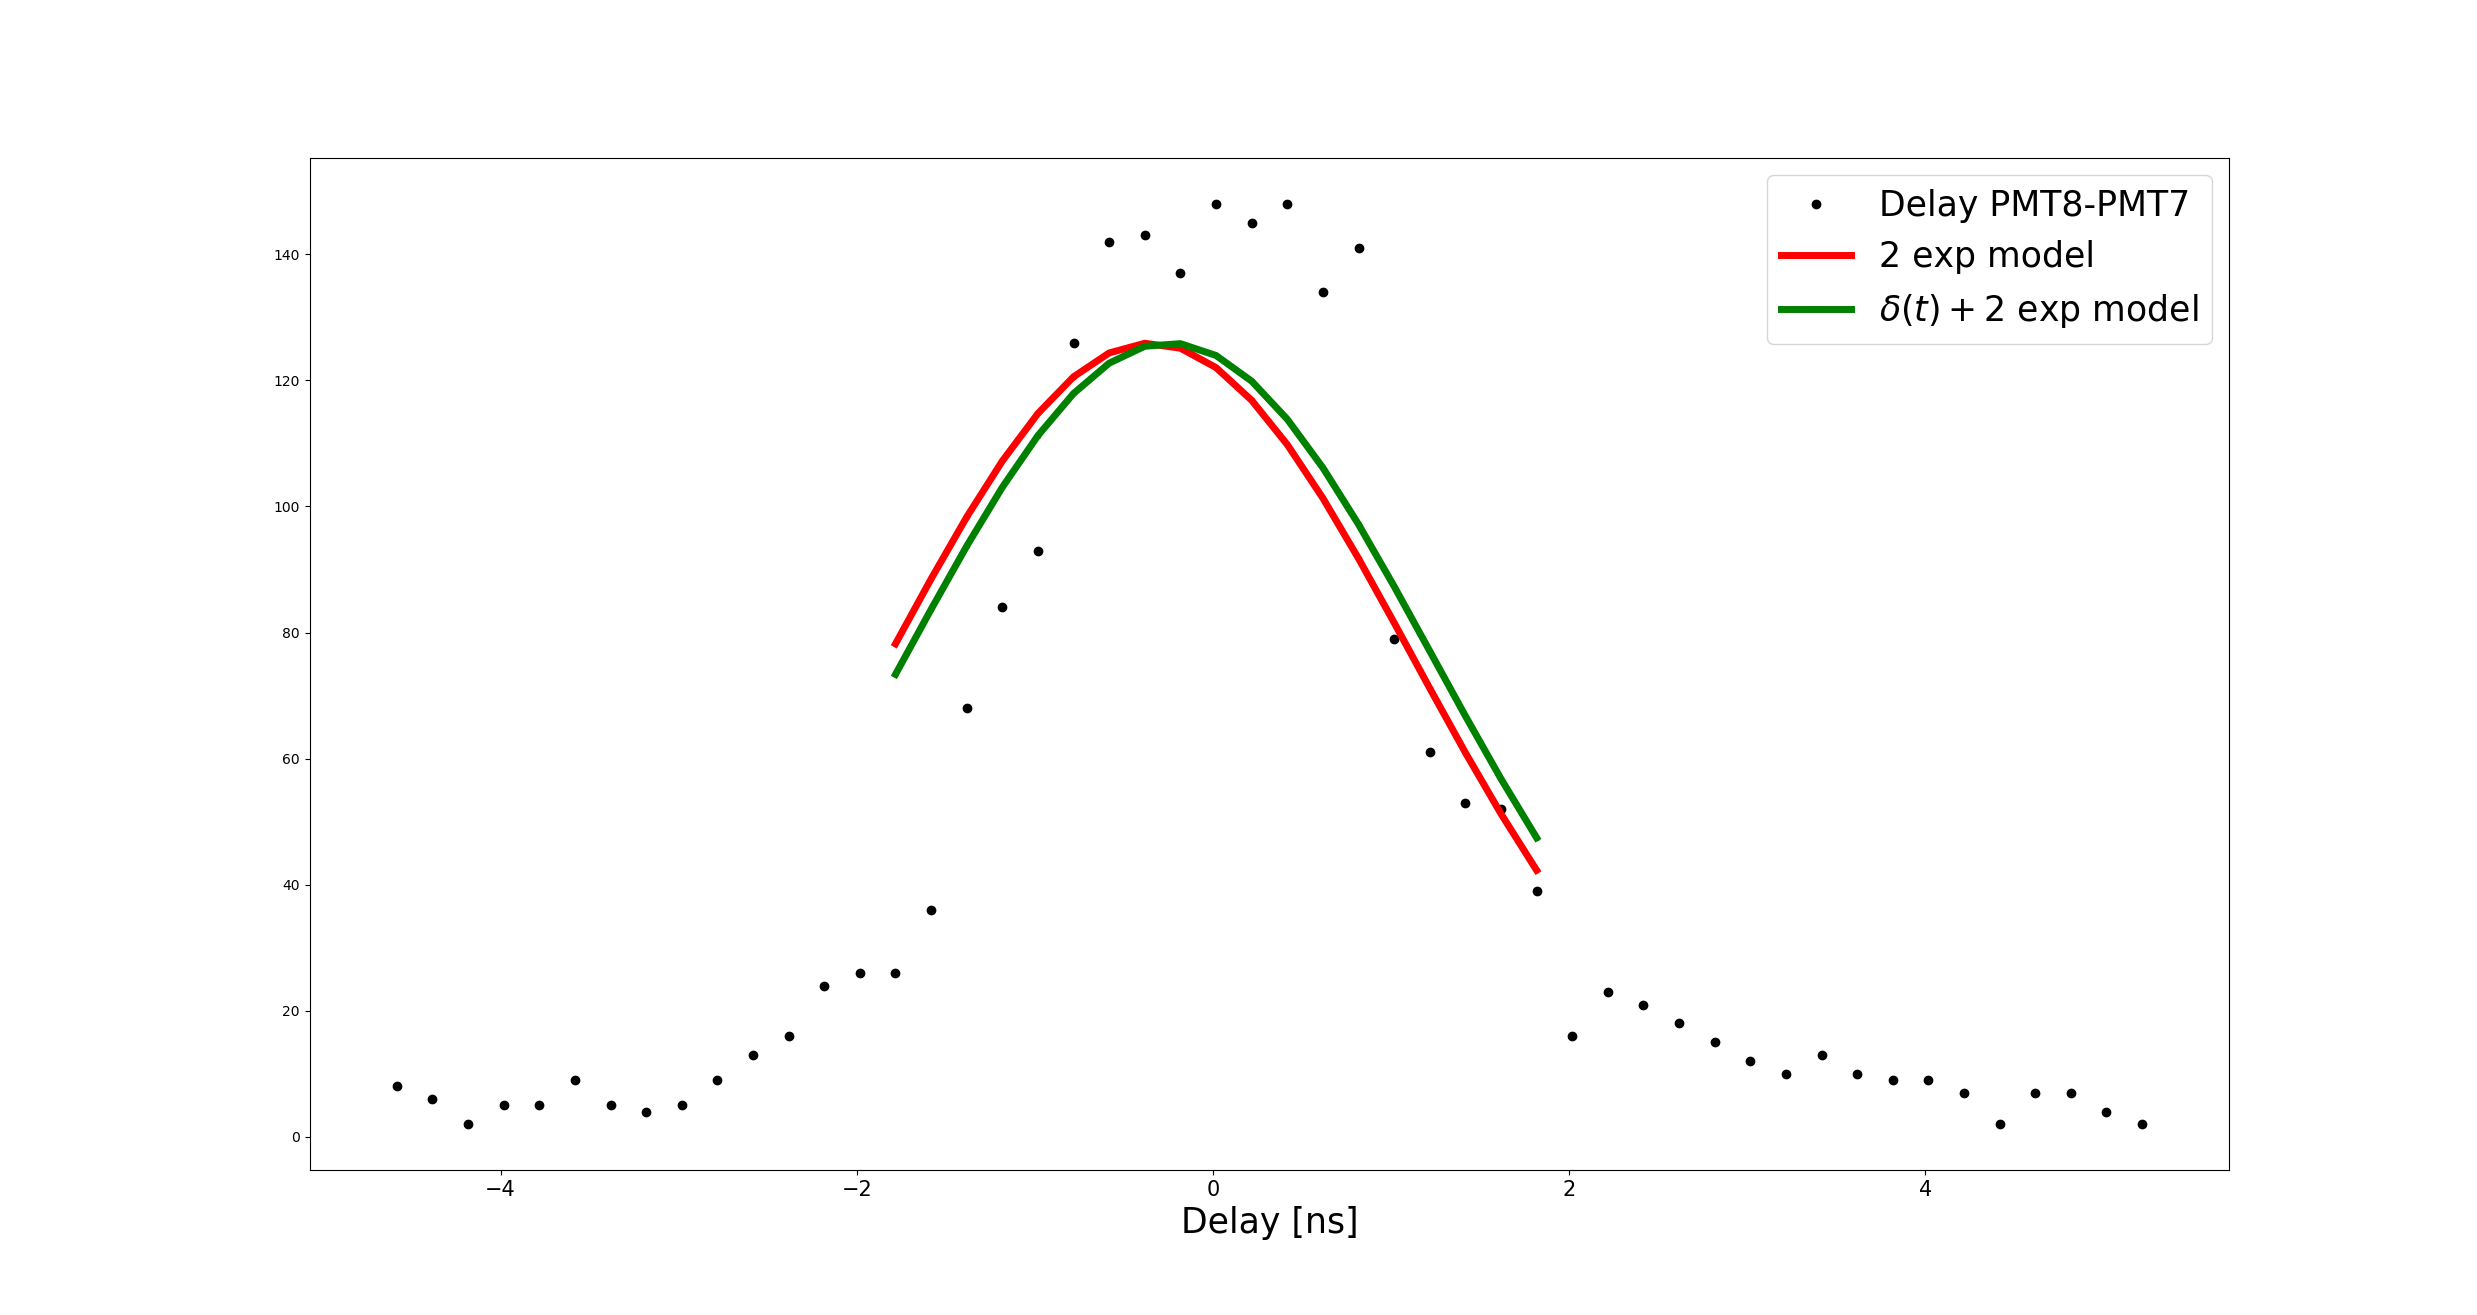
\includegraphics[width=1\textwidth]{delay_fit1.png}
\end{figure}
\end{frame}

\begin{frame}{Global Fit for the Temporal Structure the Spectra and the Delay Distribution}
\begin{figure}[h]
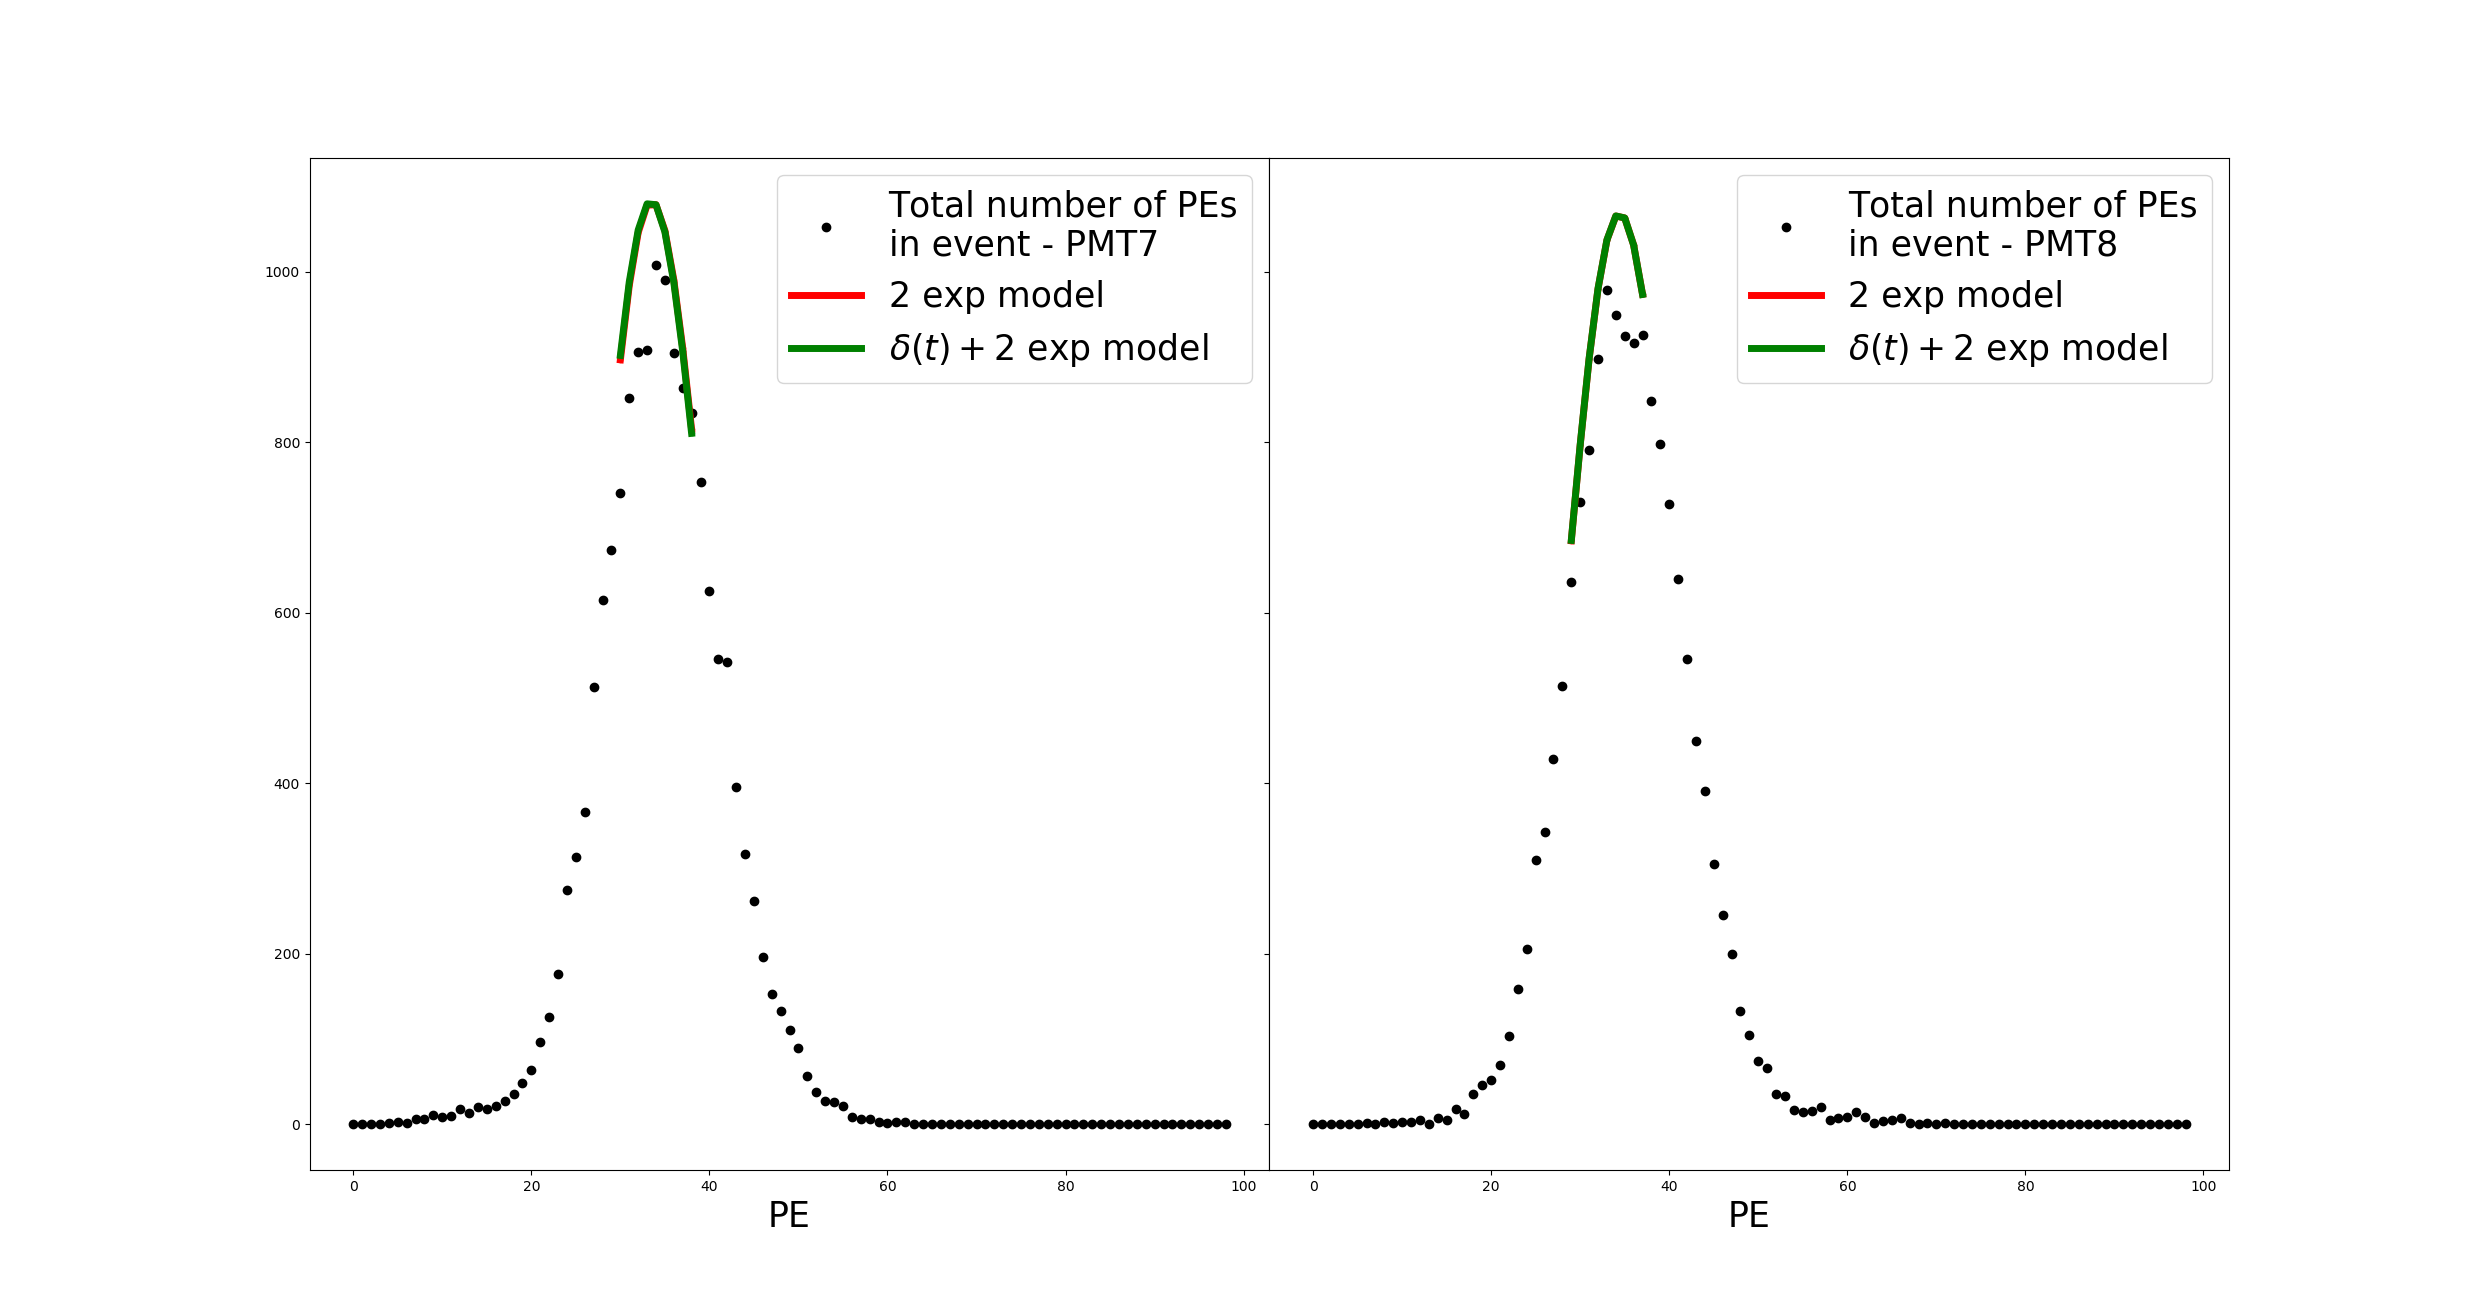
\includegraphics[width=1\textwidth]{spectra_fit1.png}
\end{figure}
\end{frame}

\begin{frame}{Global Fit for the Temporal Structure the Spectra and the Delay Distribution}
\begin{itemize}
\item Double exp model:
\begin{center}
\begin{tabular}{|c||c|c|c|c|c|c|} 
\hline
PMT & $NQ$ & $T_0$ [ns]& $\sigma_t$ [ns] & $F$ & $\tau_f$ [ns] & $\tau_s$ [ns]\\ 
\hline\hline
7 & 34 & 40 & 1.01  & 0.07 & 0.2 & 36.5 \\
\hline
8 & 35 & 39.5 & 1.08 & -- & -- & -- \\
\hline
\end{tabular}
\end{center} 

\item $\delta(t)+$ double exp model:
\begin{center}
\begin{tabular}{|c||c|c|c|c|c|c|c|} 
\hline
PMT & $NQ$ & $T_0$ [ns]& $\sigma_t$ [ns] & $R$ & $F$ & $\tau_f$ [ns] & $\tau_s$ [ns]\\ 
\hline\hline
7 & 36 & 45.3 & 0.97 & 0.06  & 0.7 & 30 & 100 \\
\hline
8 & 37 & 35.1 & 1.1& 0.07 & -- & -- & -- \\
\hline
\end{tabular}
\end{center} 
\end{itemize}
\end{frame}

\begin{frame}{Dark Count Correction}
The reconstruction algorithm some time reconstruct a PE where it should not be. The rate of this falls reconstructions is the dark count ($f_{dc}$). The probability to have $n>0$ dark PEs at a digi point is $f_{dc}^n$ and the probability to have 0 dark PEs in a digi point is $1-\frac{f_{dc}}{1-f_{dc}}$. This parameter can be calibrated from the pulser data by applying the reconstruction algorithm out of the time window where the SPE is expected.
\begin{figure}[h]
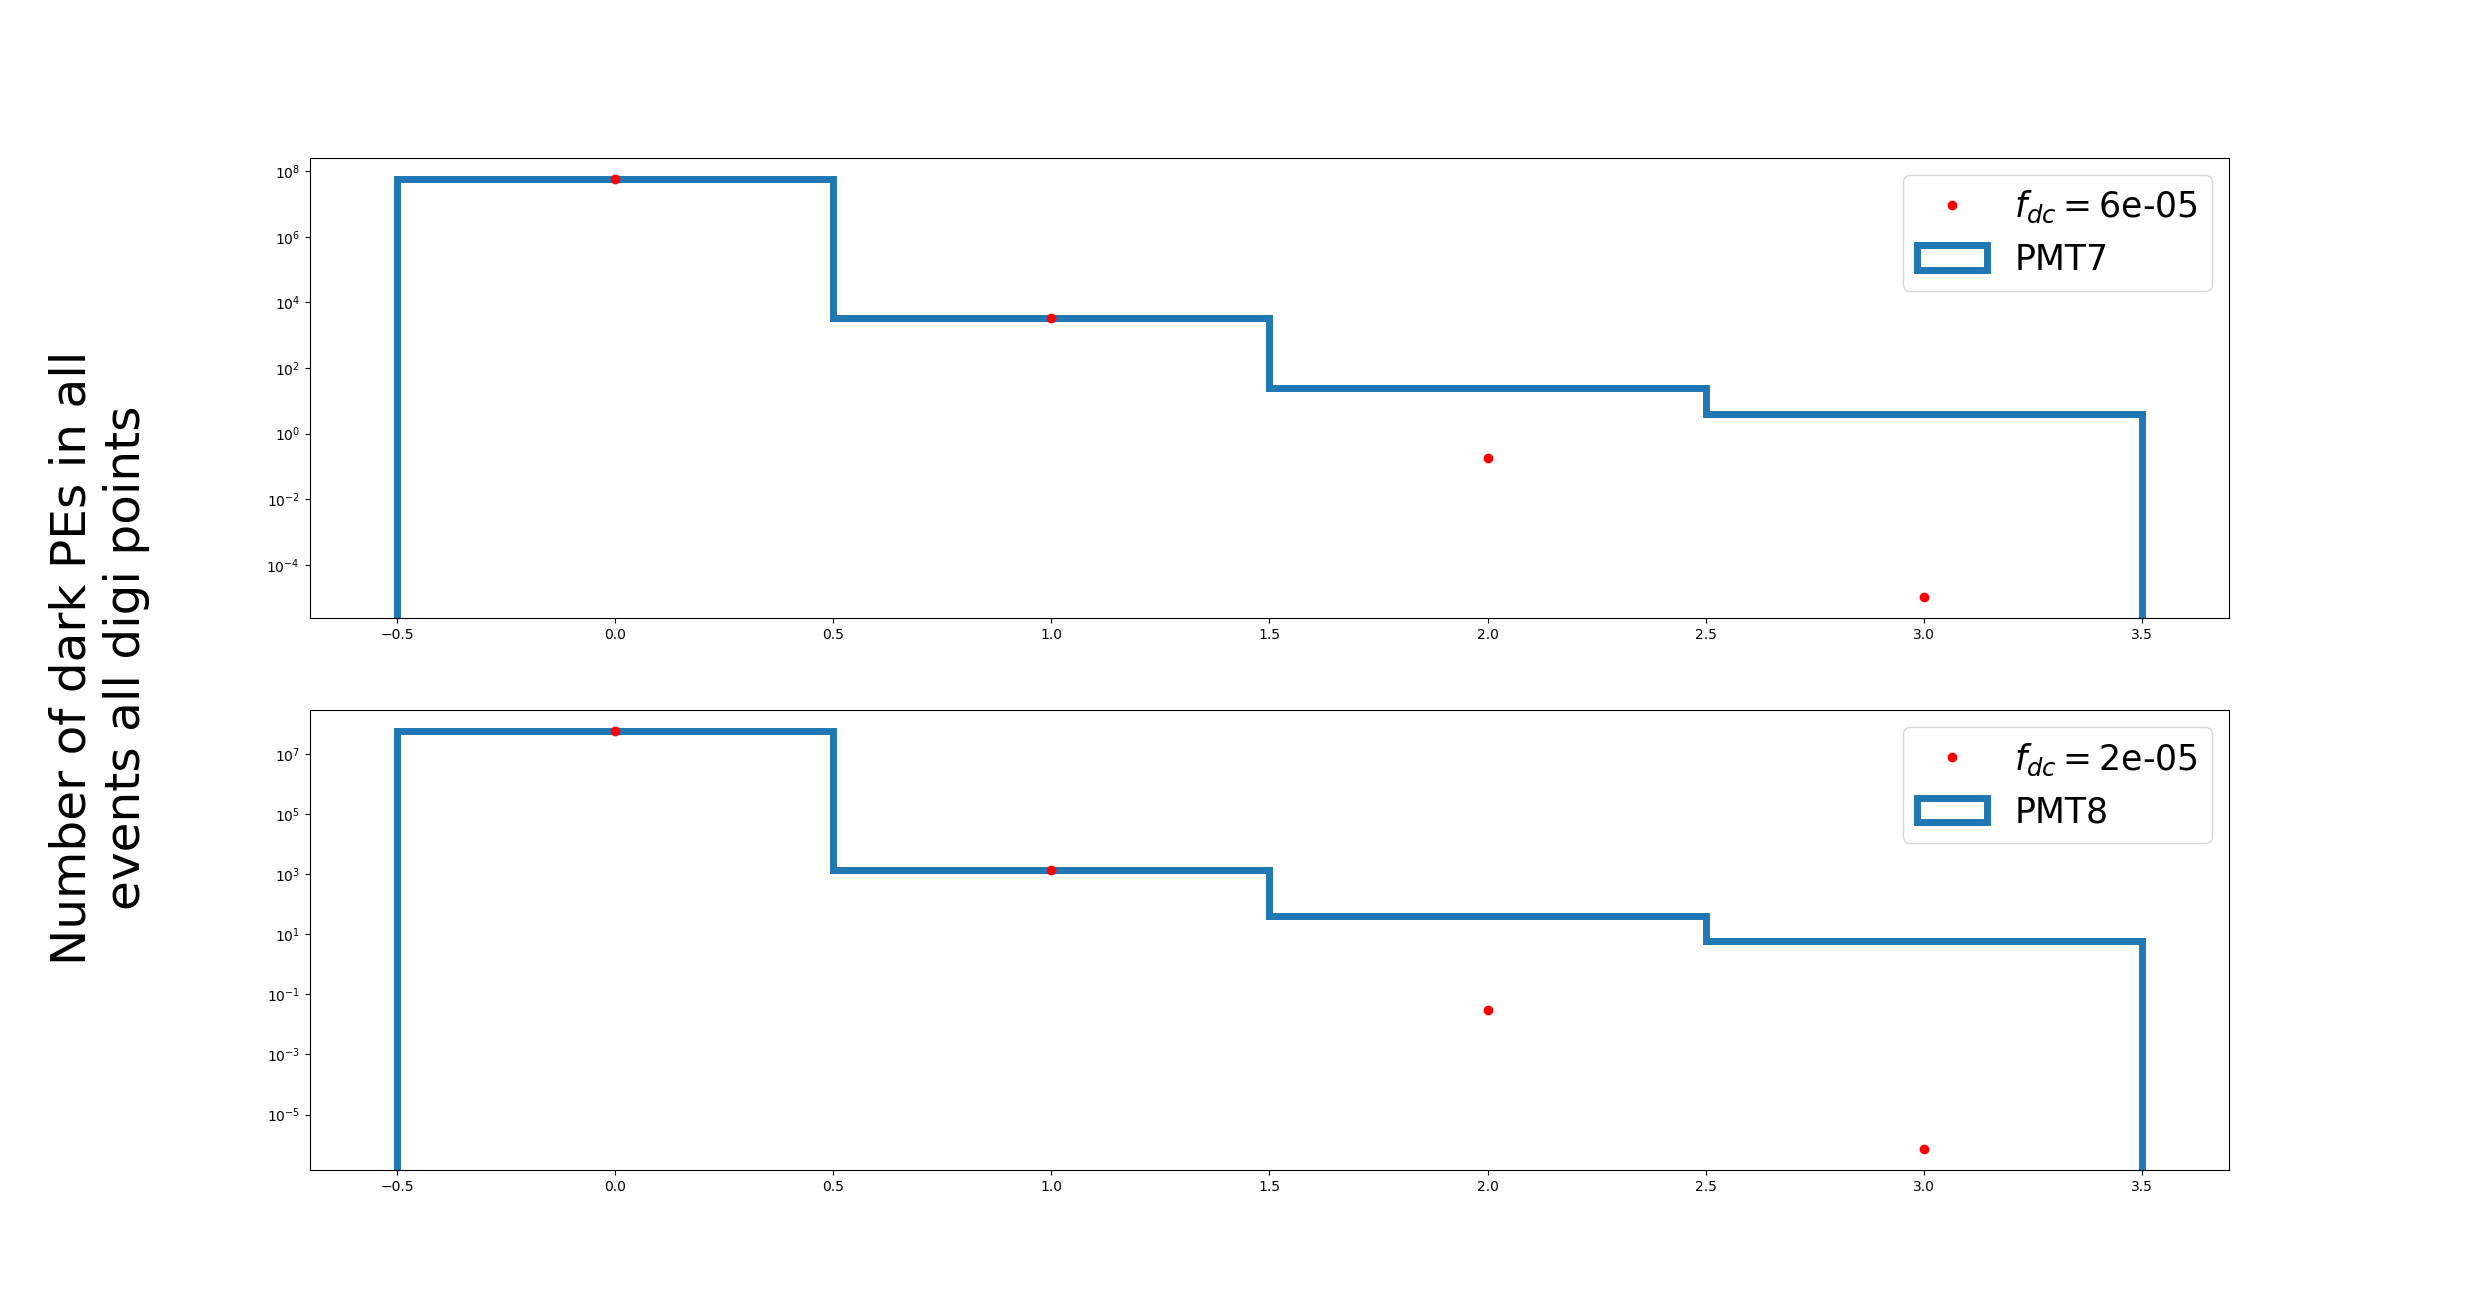
\includegraphics[width=0.75\textwidth]{f_dc.png}
\end{figure}
\end{frame}

\begin{frame}{Dark Count Correction to the Model}
\begin{equation}
\begin{split}
\tilde{H}_{0i}&\rightarrow \left(1-\frac{f_{dc}}{1-f_{dc}}\right)\tilde{H}_{0i}\\
\tilde{H}_{0i}&\rightarrow \left(1-\frac{f_{dc}}{1-f_{dc}}\right)\tilde{H}_{ni}+\sum_{m=1}^{n}f_{dc}^m\tilde{H}_{n-mi}
\end{split}
\end{equation}
This should be corrected before the alignment.
\end{frame}


\begin{frame}{Dark Count Correction to the Simulation}
For each digi point add a random number sampled with the probability
\begin{equation}
\begin{split}
&P(0)=1-\frac{1}{1-f_{dc}}\\
&P(n>0)=f_{dc}^n
\end{split}
\end{equation}
\end{frame}

\begin{frame}{Correction due the SPE Area Resolution}
When $n$ PEs created at some time in the PMT there is some probability that $m\neq n$ PEs will be resolved. This is related to the SPE area resolution. 

\begin{figure}[h]
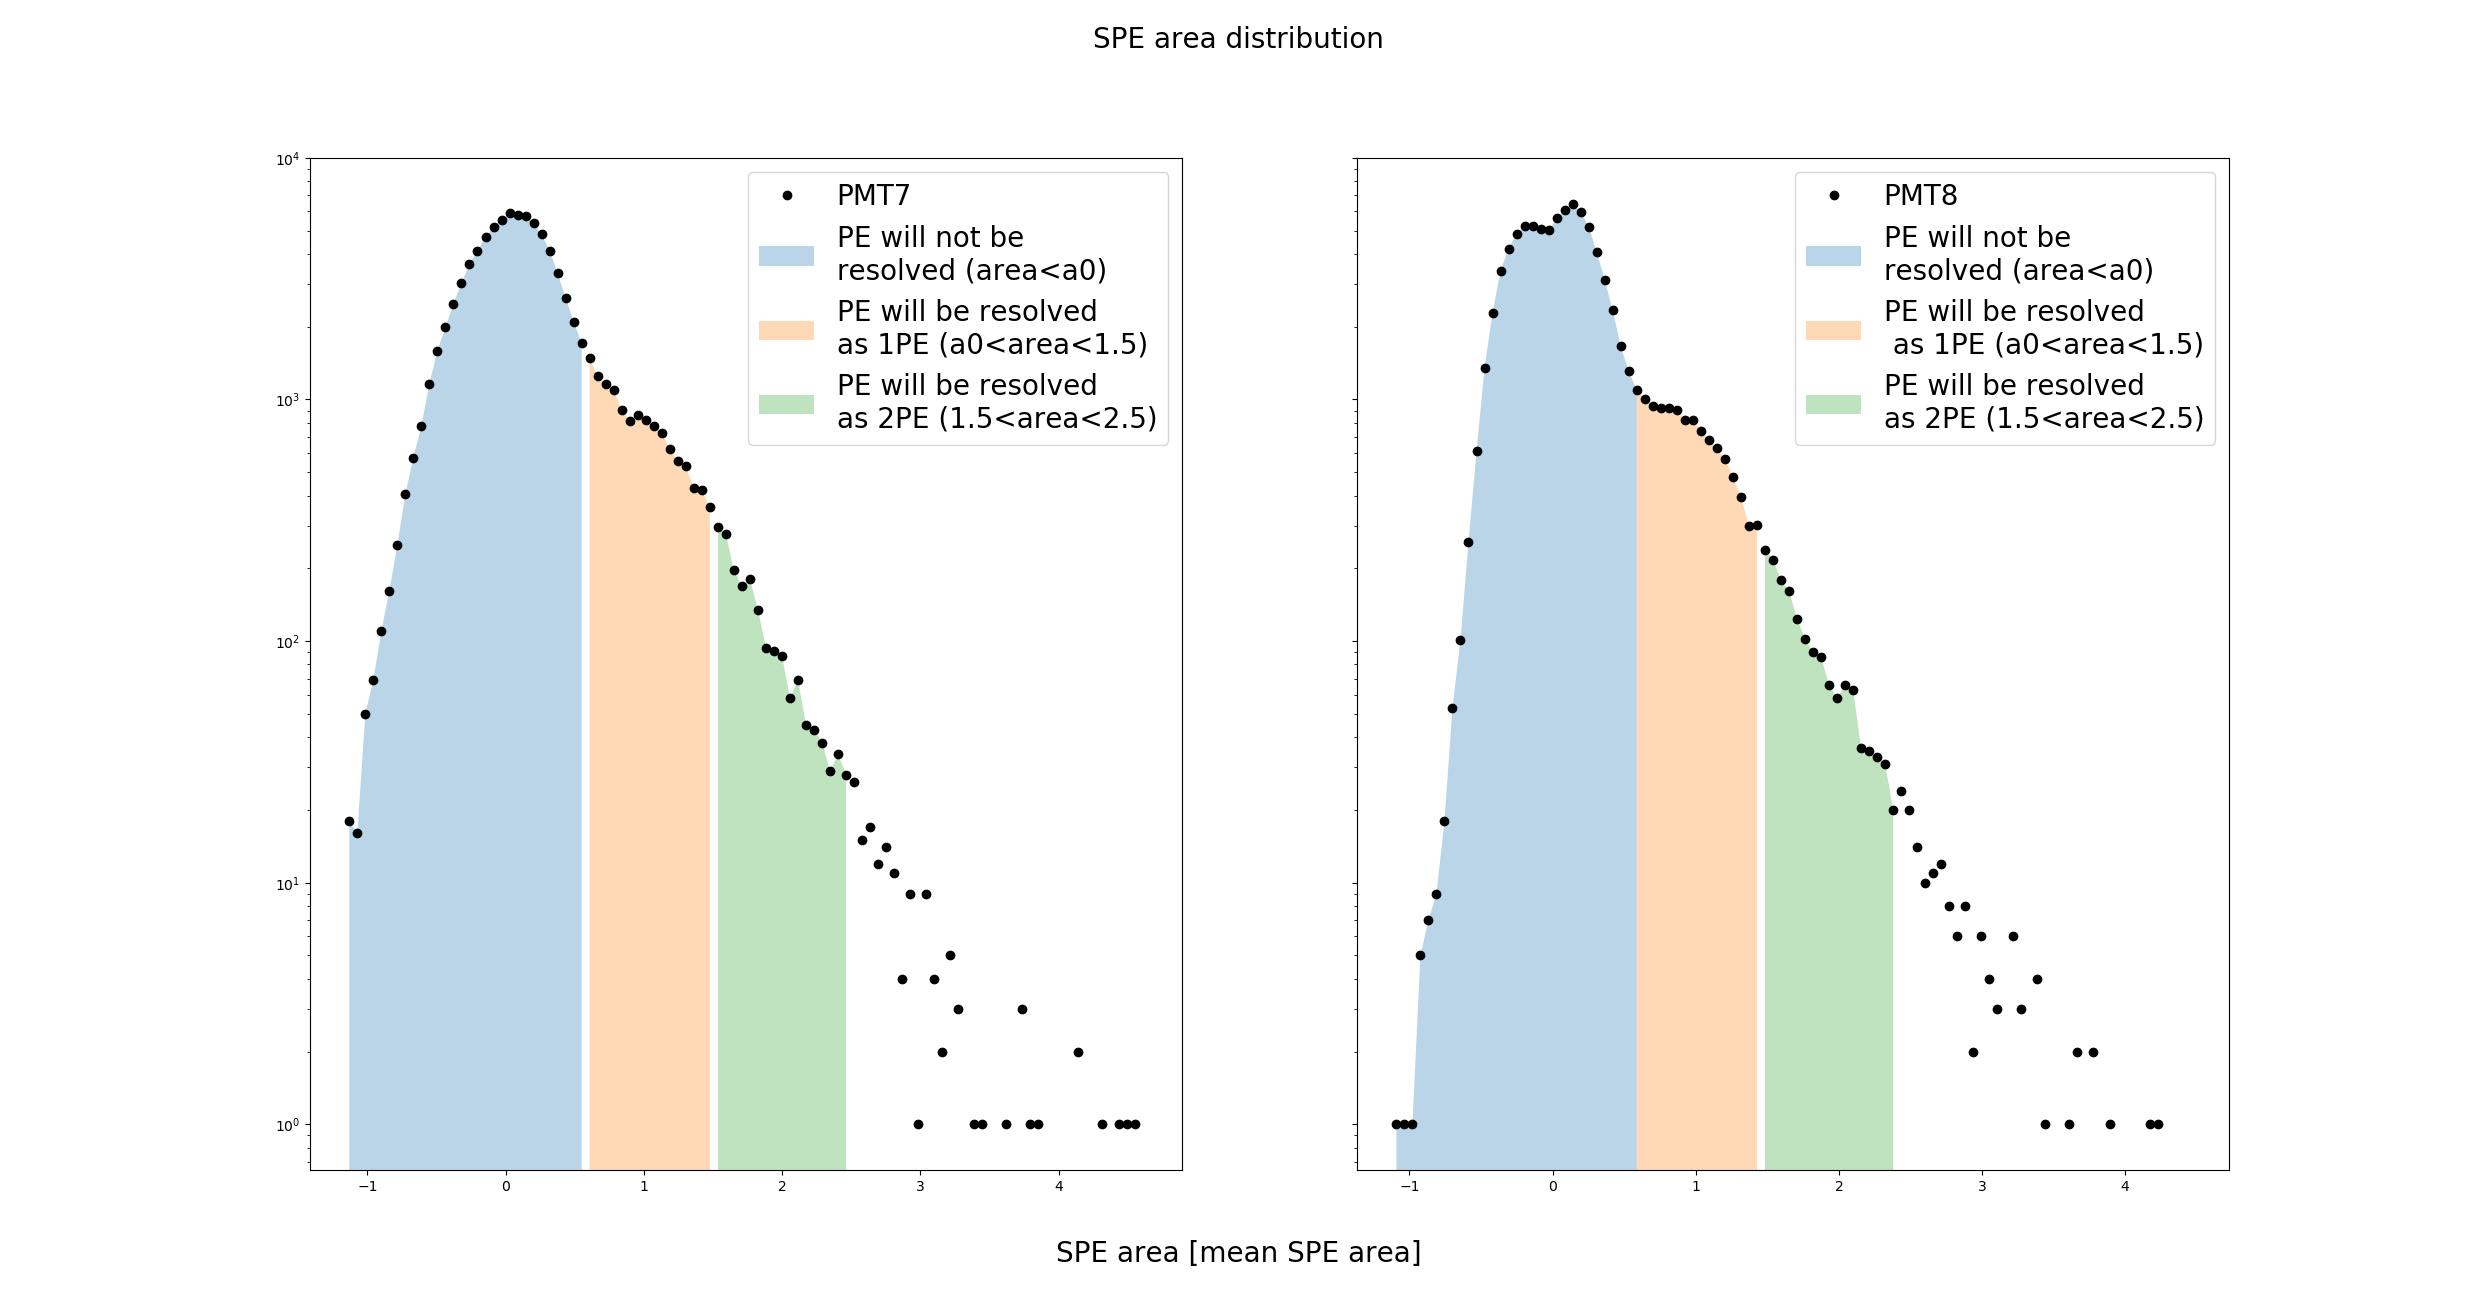
\includegraphics[width=0.75\textwidth]{SPE_area.png}
\end{figure}

$\mu_{pad}$ and $\sigma_{pad}$ are the mean and width of the padestial distribution, $\sigma_{spe}$ is the width of the SPE area distribution (around 1) and $a_0$ is some threshold area which under it the PE will not be resolved. 
\end{frame}

\begin{frame}{Correction to the Simulation due the SPE Area Resolution}
For each non-dark PE assign an area chosen randomly from $\text{Normal}\left(\text{mean}=\mu_{pad}+1, \sigma^2=\sigma_{pad}^2+\sigma_{spe}^2\right)$.\\
\begin{itemize}
\item If the area$<a_0$ eraser this PE.\\
\item If the $a_0<$area$<1.5$ leave the PE.\\
\item If the $n-0.5<$area$<n+0.5$ PE$\rightarrow n$PEs.
\end{itemize}

\end{frame}


\begin{frame}{Correction to the Model due the SPE Area Resolution}
Recall that $\tilde{H}_{ni}$ is the number of times $n$ PEs should be resolved at time $t_i$.
$H_{ni}=\sum_mP_{nm}\tilde{H}_{mi}$ is the probability to resolve $n$ PEs at time $t_i$, where $P_{nm}$ is the probability to resolve $n$ PEs from $m$ real PEs.\\
\begin{itemize}
\item $P_{n0}=\delta_{n0}$ because the probability to resolve $n$ PEs from 0 PEs is accounted by the dark count.
\item $P_{0m}=\frac{1}{\sqrt{2\pi\left(\sigma_{pad}^2+m\sigma_{spe}^2\right)}}\int_{-\infty}^{a_0}e^{-\frac{\left((x-(\mu_{pad}+m)\right)^2}{2\left(\sigma_{pad}^2+m\sigma_{spe}^2\right)}}dx$\\
\item $P_{1m}=\frac{1}{\sqrt{2\pi\left(\sigma_{pad}^2+m\sigma_{spe}^2\right)}}\int_{a_0}^{1.5}e^{-\frac{\left((x-(\mu_{pad}+m)\right)^2}{2\left(\sigma_{pad}^2+m\sigma_{spe}^2\right)}}dx$\\
\item $P_{nm}=\frac{1}{\sqrt{2\pi\left(\sigma_{pad}^2+m\sigma_{spe}^2\right)}}\int_{n-0.5}^{n+0.5}e^{-\frac{\left((x-(\mu_{pad}+m)\right)^2}{2\left(\sigma_{pad}^2+m\sigma_{spe}^2\right)}}dx$\\
\end{itemize}
\end{frame}

\begin{frame}{Global Fit of the Temporal Structure, Delay, Spectra, Dark Count rate and SPE Area Distribution}
\begin{figure}[h]
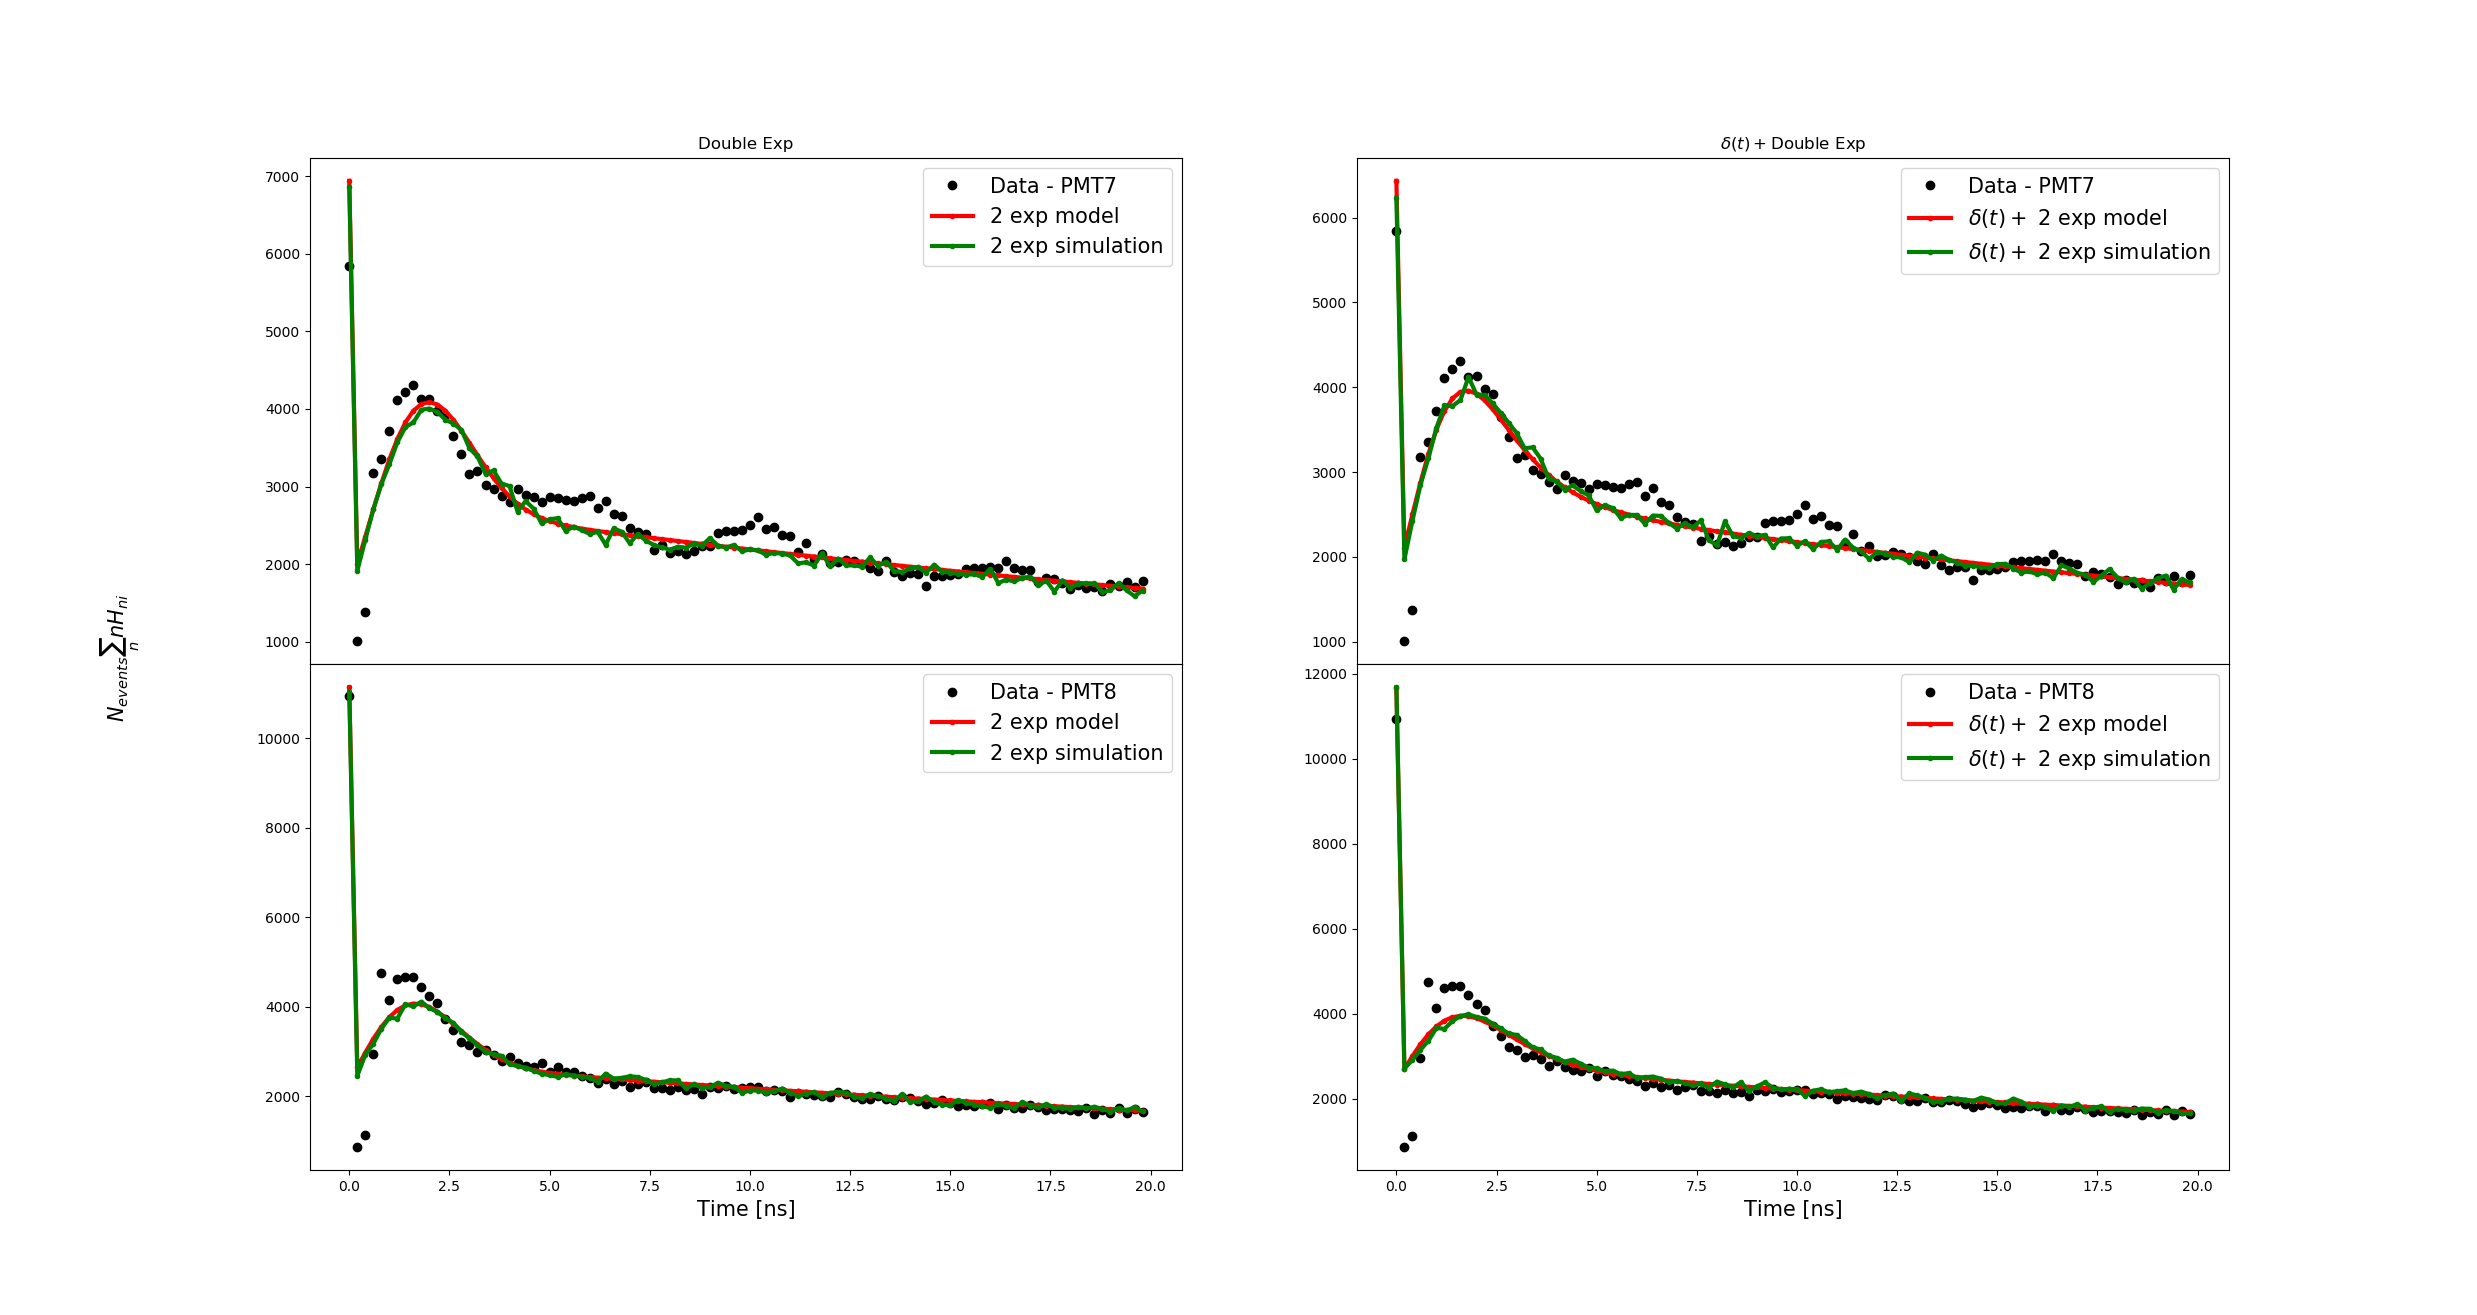
\includegraphics[width=1\textwidth]{data_fit.png}
\end{figure}
\end{frame}

\begin{frame}{Global Fit of the Temporal Structure, Delay, Spectra, Dark Count rate and SPE Area Distribution}
\begin{figure}[h]
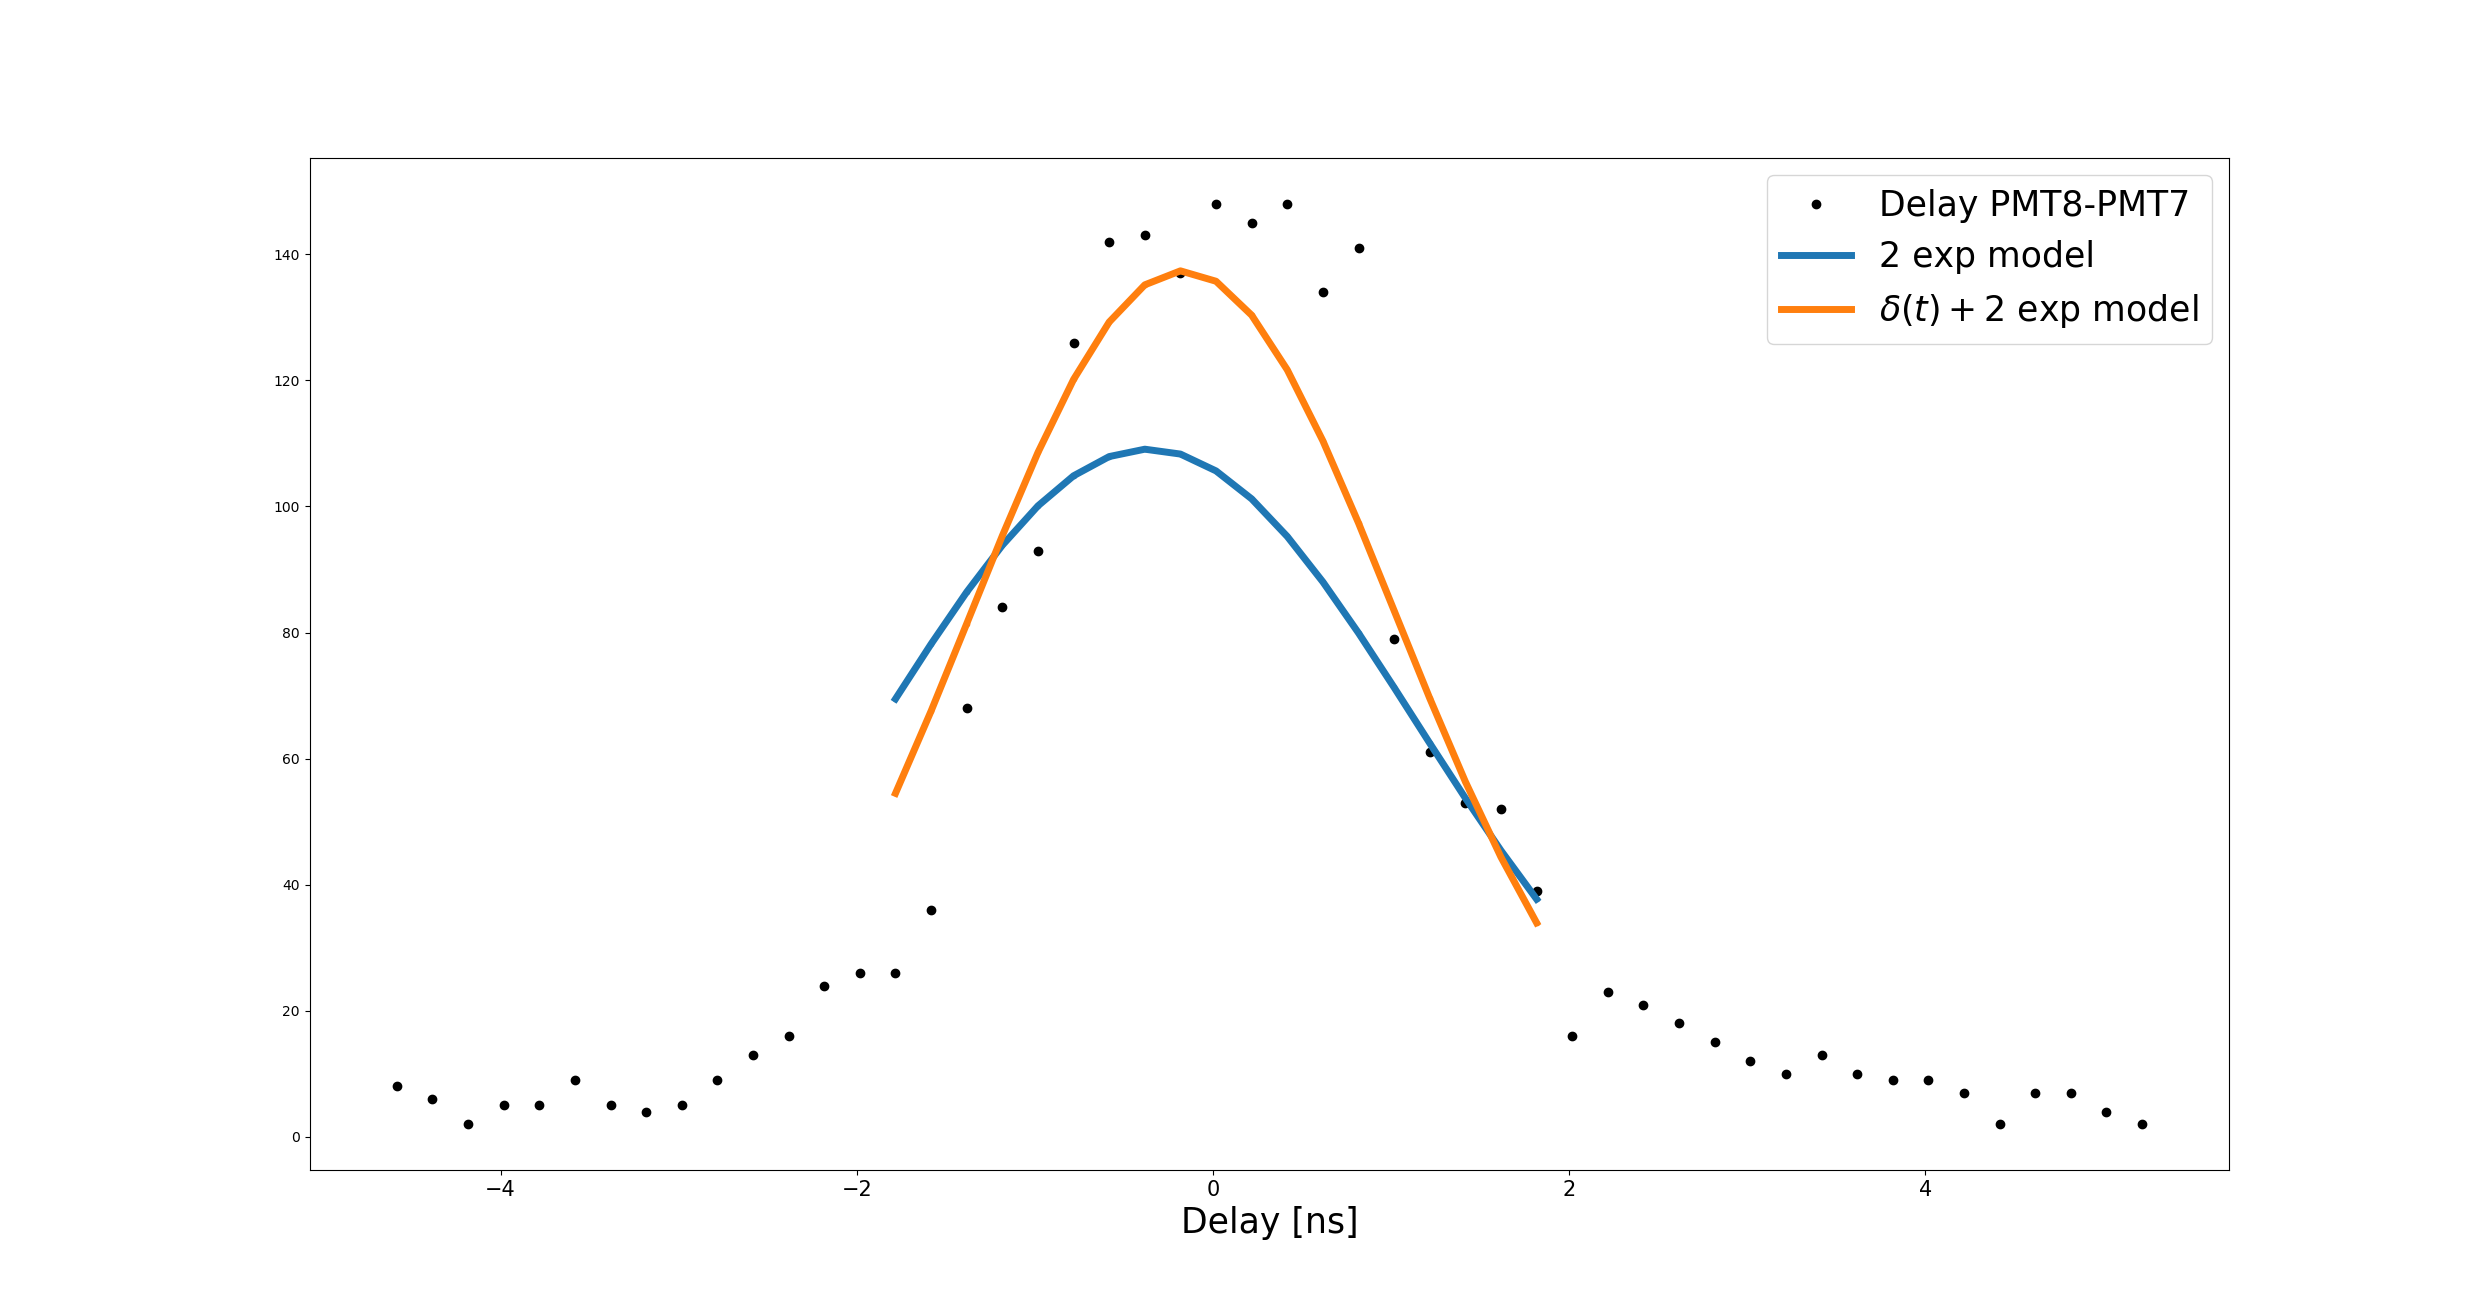
\includegraphics[width=1\textwidth]{delay_fit.png}
\end{figure}
\end{frame}

\begin{frame}{Global Fit of the Temporal Structure, Delay, Spectra, Dark Count rate and SPE Area Distribution}
\begin{figure}[h]
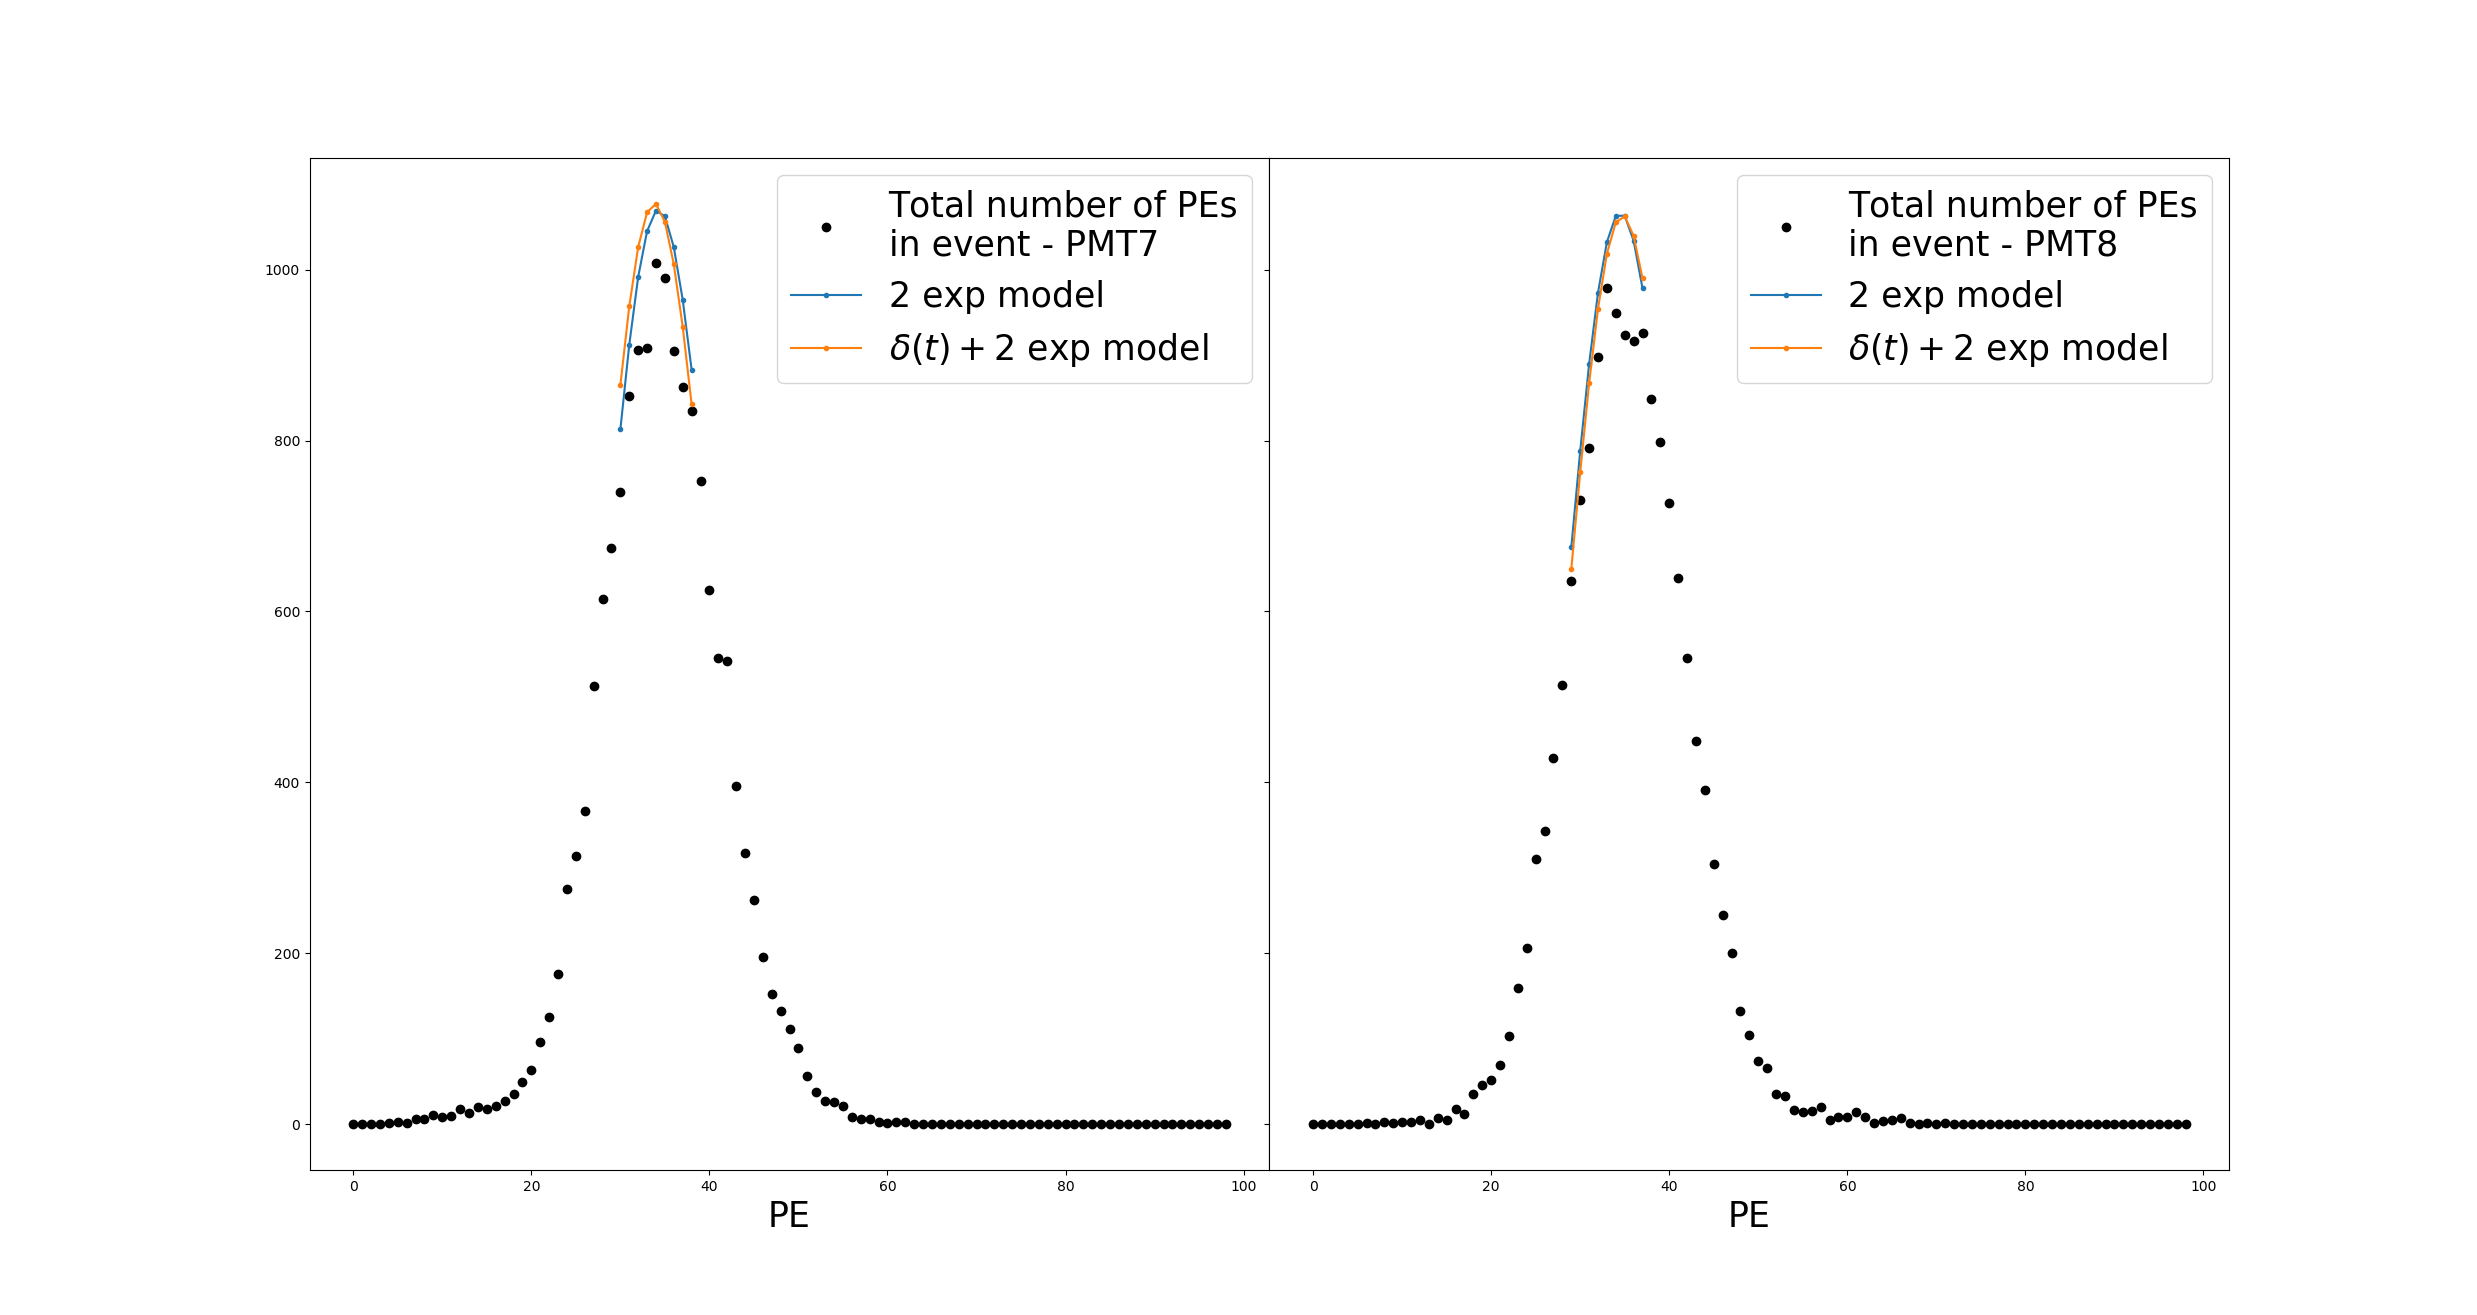
\includegraphics[width=1\textwidth]{spectra_fit.png}
\end{figure}
\end{frame}

\begin{frame}{Global Fit of the Temporal Structure, Delay, Spectra, Dark Count rate and SPE Area Distribution}
\begin{figure}[h]
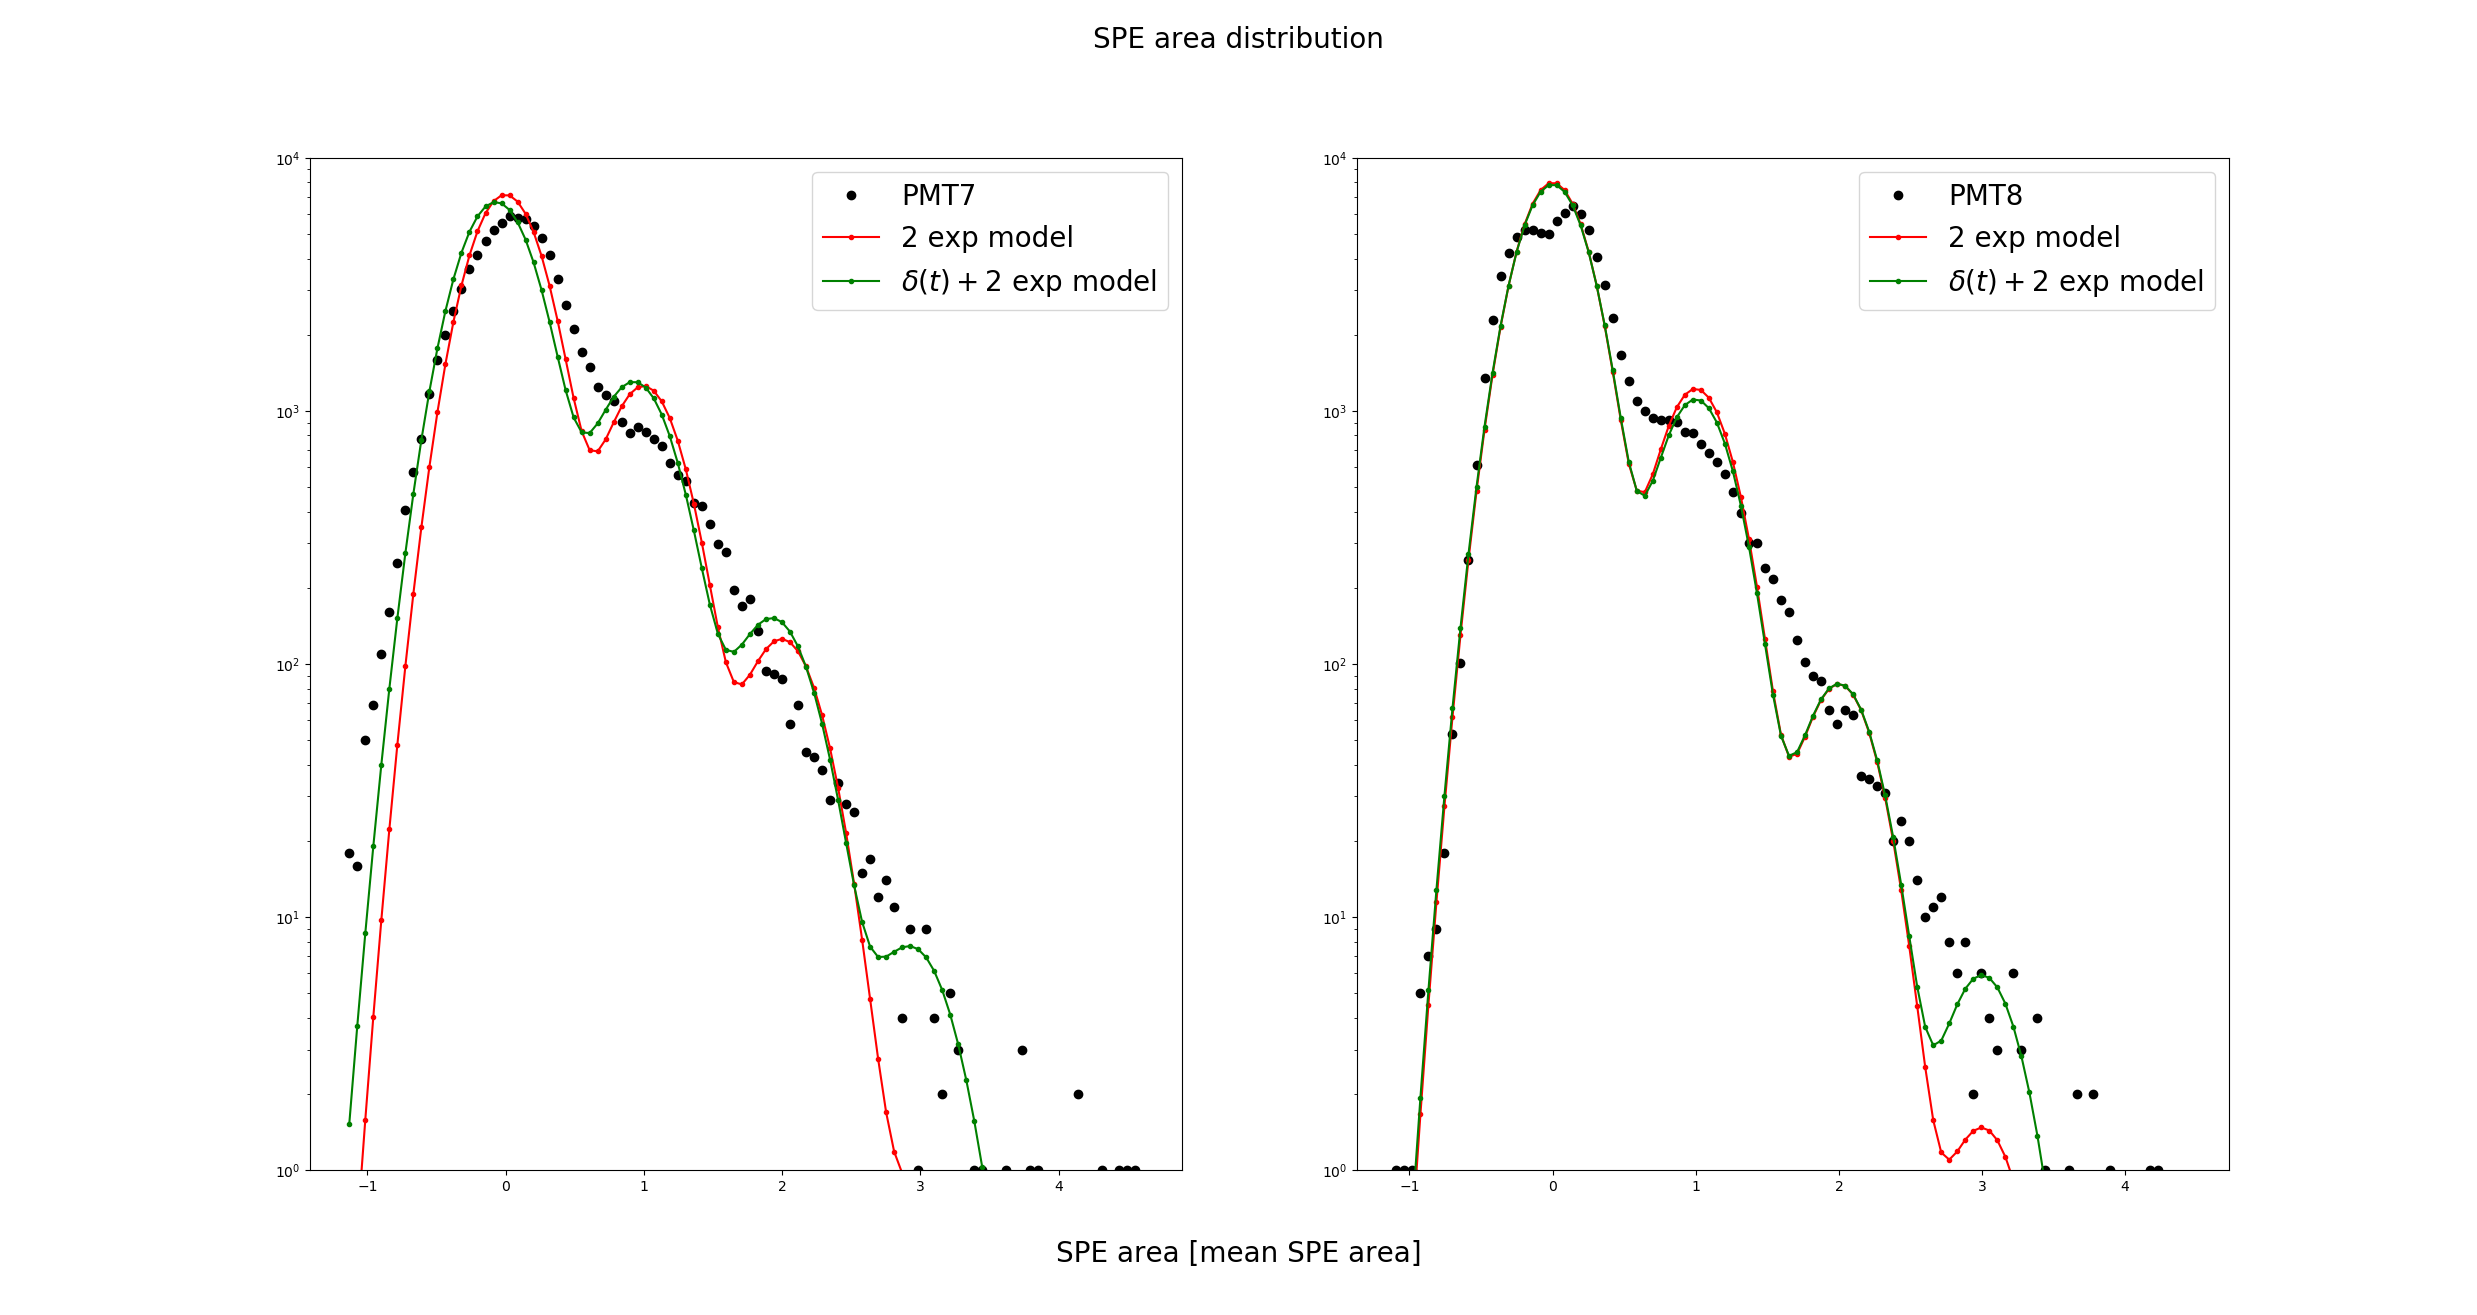
\includegraphics[width=1\textwidth]{area_fit.png}
\end{figure}
The global fit prefers a more narrow area distribution than the actual pulser data.
\end{frame}

\begin{frame}{Global Fit of the Temporal Structure, Delay, Spectra, Dark Count rate and SPE Area Distribution}
\begin{figure}[h]
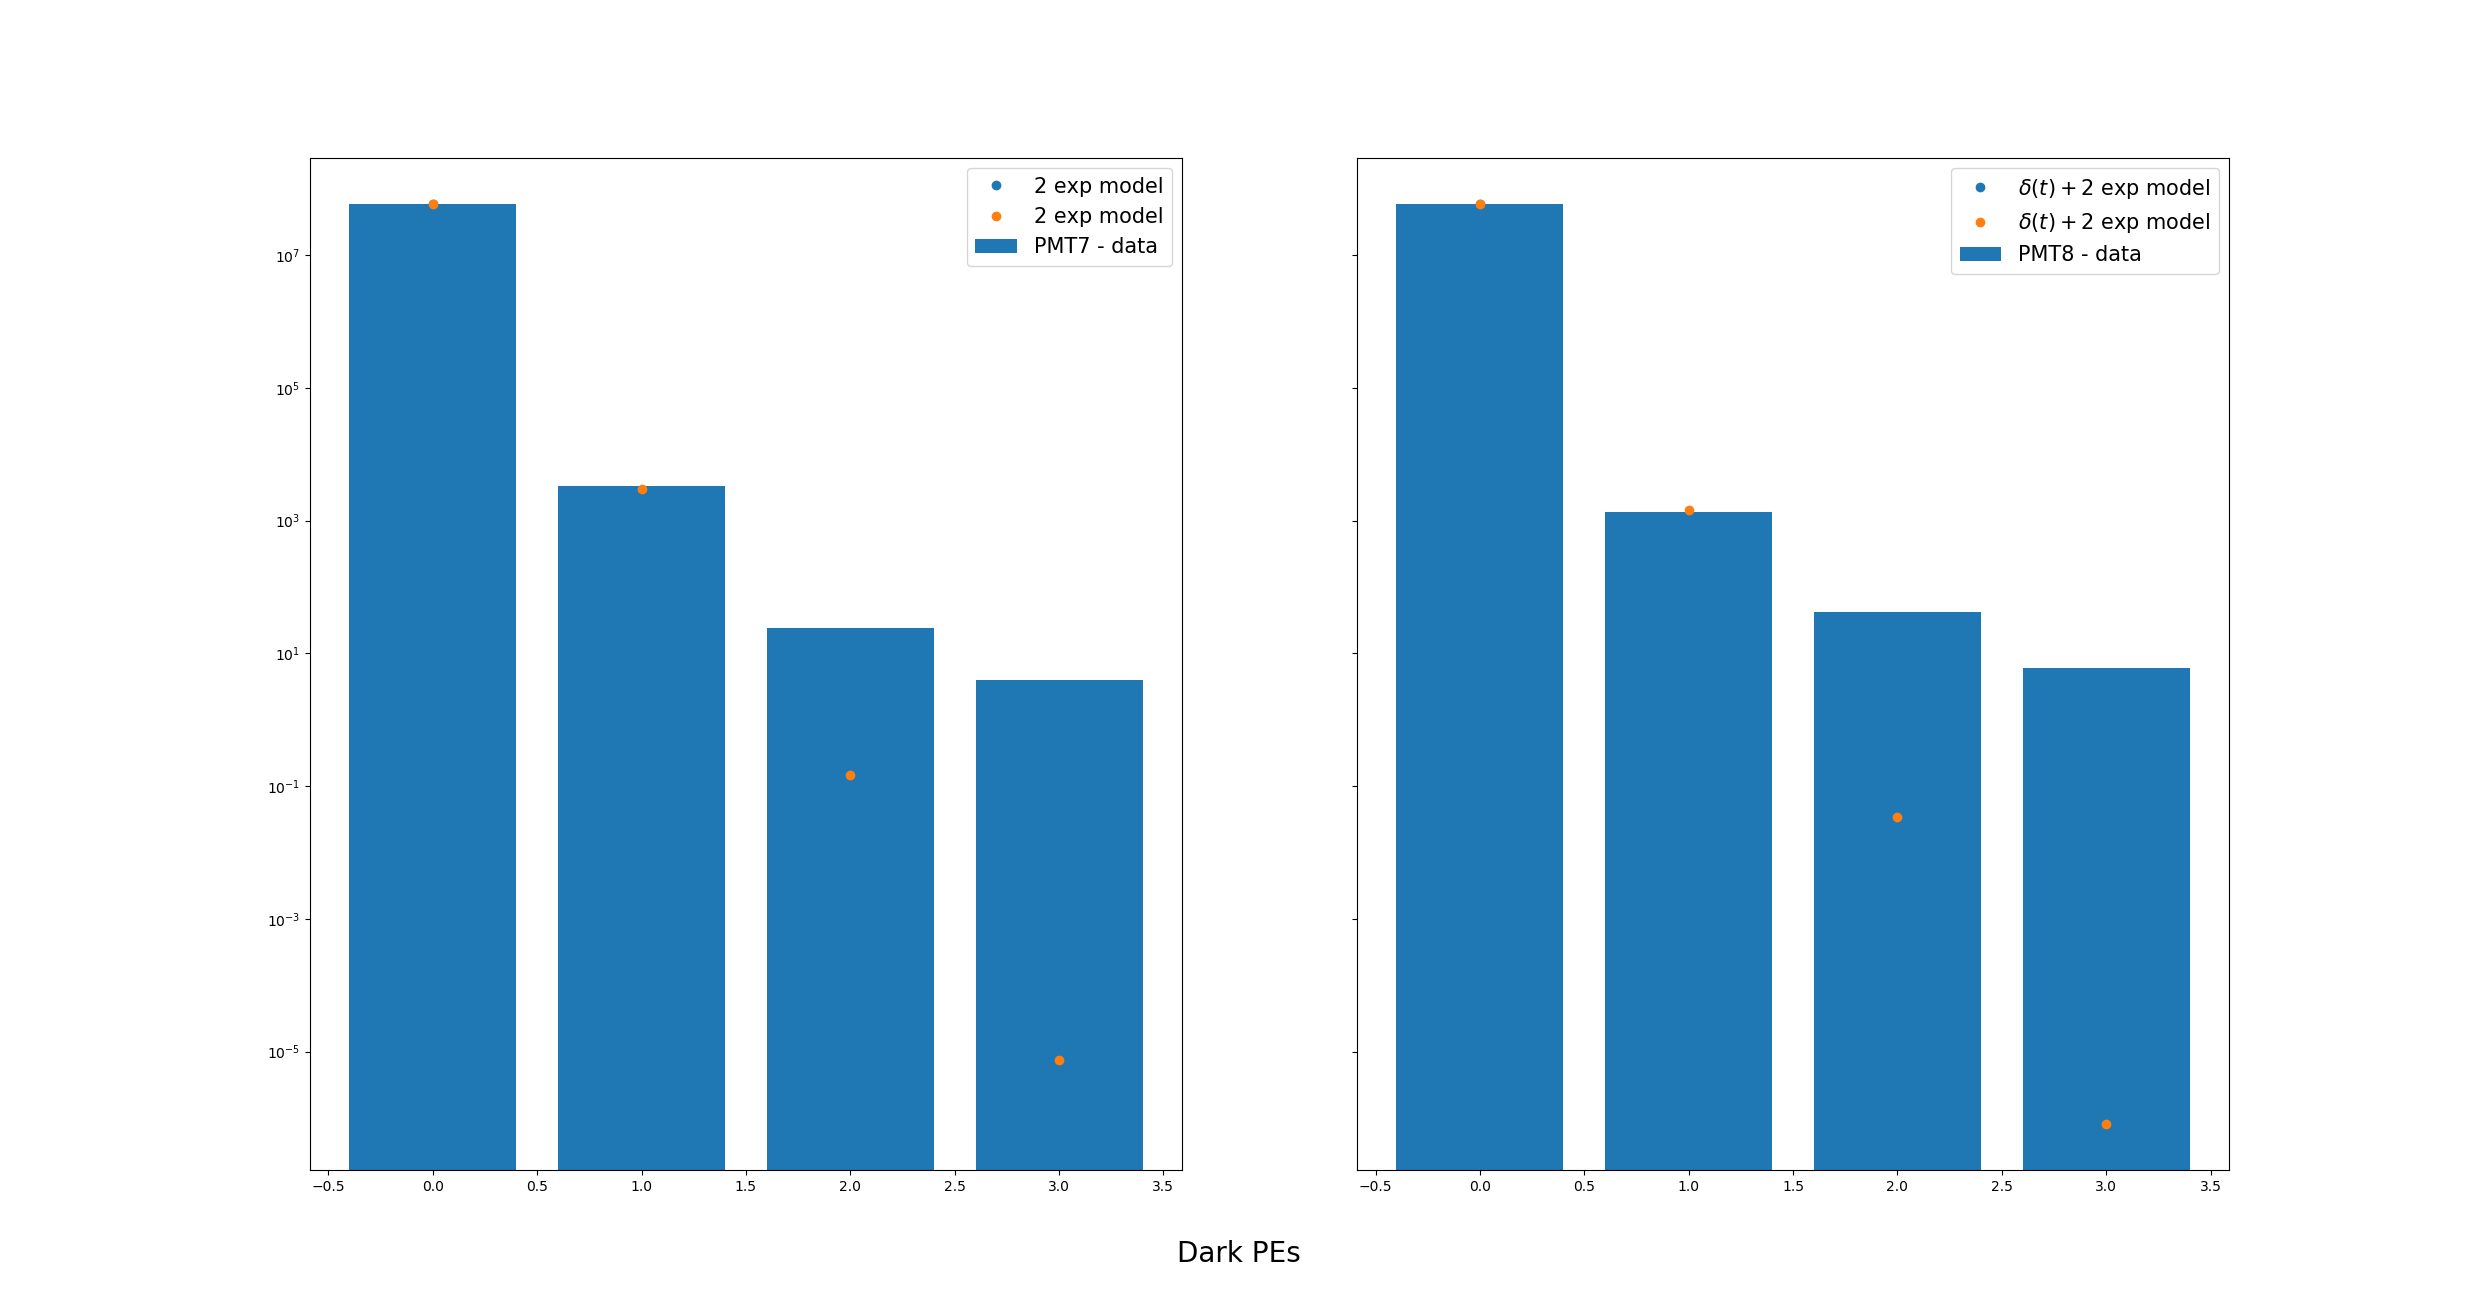
\includegraphics[width=1\textwidth]{DC_fit.png}
\end{figure}
\end{frame}

\begin{frame}{Global Fit for the Temporal Structure the Spectra and the Delay Distribution}
\begin{center}
\begin{tabular}{|c|c|c|c|} 
\hline
model & $F$ & $\tau_f$ [ns] & $\tau_s$ [ns]\\ 
\hline\hline
2 exp model & 0.07 & 0.2 & 36\\
\hline
$\delta(t)+$ 2 exp model& 0.05 & 1.1 & 36\\
\hline
\end{tabular}
\end{center} 
\end{frame}

\end{document}

